\documentclass[a4paper]{article}
\usepackage{vntex}
\usepackage{wrapfig}
\usepackage{graphicx}
%\usepackage[english,vietnam]{babel}
%\usepackage[utf8]{inputenc}

%\usepackage[utf8]{inputenc}
%\usepackage[francais]{babel}
\usepackage{a4wide,amssymb,epsfig,latexsym,array,hhline,fancyhdr}
\usepackage[normalem]{ulem}
%\usepackage{soul}

\usepackage{ upgreek }
\usepackage[makeroom]{cancel}
\usepackage{amsmath}
\usepackage{amsthm}
\usepackage{multicol,longtable,amscd}
\usepackage{diagbox}%Make diagonal lines in tables
\usepackage{booktabs}
\usepackage{alltt}
\usepackage[framemethod=tikz]{mdframed}% For highlighting paragraph backgrounds
\usepackage{caption,subcaption}

\usepackage{lastpage}
\usepackage[lined,boxed,commentsnumbered]{algorithm2e}
\usepackage{enumerate}
\usepackage{color}
\usepackage{graphicx}						% Standard graphics package
\usepackage{array}
\usepackage{tabularx, caption}
\usepackage{tipa}
\usepackage{multirow}
\usepackage{multicol}
\usepackage{hhline}
\usepackage{rotating}
\usepackage{graphics}
\usepackage{geometry}
\usepackage{setspace}
\usepackage{tcolorbox}
\usepackage{listings}
\usepackage{epsfig}
\usepackage{tikz}
\usepackage{xurl}
\usetikzlibrary{arrows,snakes,backgrounds}
\usepackage[unicode]{hyperref}
\hypersetup{urlcolor=blue,linkcolor=black,citecolor=black,colorlinks=true} 
%\usepackage{pstcol} 								% PSTricks with the standard color package

\usepackage[normalem]{ulem}



\def\thesislayout{	% A4: 210 × 297
	\geometry{
		a4paper,
		total={160mm,240mm},  % fix over page
		left=30mm,
		top=30mm,
	}
}
\thesislayout

%\usepackage{fancyhdr}
\setlength{\headheight}{40pt}
\pagestyle{fancy}
\fancyhead{} % clear all header fields
\fancyhead[L]{
 \begin{tabular}{rl}
    \begin{picture}(25,15)(0,0)
    \put(0,-8){
\includegraphics[width=8mm, height=8mm]{BK.png}}
    %\put(0,-8){\epsfig{width=10mm,figure=hcmut.eps}}
   \end{picture}&
	%\includegraphics[width=8mm, height=8mm]{hcmut.png} & %
	\begin{tabular}{l}
		\textbf{\bf \ttfamily Trường Đại Học Bách Khoa Tp.Hồ Chí Minh}\\
		\textbf{\bf \ttfamily Khoa Khoa Học \& Kỹ Thuật Máy Tính}
	\end{tabular} 	
 \end{tabular}
}
\fancyhead[R]{
	\begin{tabular}{l}
		\tiny \bf \\
		\tiny \bf 
	\end{tabular}  }
\fancyfoot{} % clear all footer fields
\fancyfoot[L]{\scriptsize \ttfamily Bài tập lớn môn Công Nghệ Phần Mềm (CO3001) - Niên khóa 2022-2023}
\fancyfoot[R]{\scriptsize \ttfamily Trang {\thepage}/\pageref{LastPage}}
\renewcommand{\headrulewidth}{0.3pt}
\renewcommand{\footrulewidth}{0.3pt}


%%%
\setcounter{secnumdepth}{4}
\setcounter{tocdepth}{3}
\makeatletter
\newcounter {subsubsubsection}[subsubsection]
\renewcommand\thesubsubsubsection{\thesubsubsection .\@alph\c@subsubsubsection}
\newcommand\subsubsubsection{\@startsection{subsubsubsection}{4}{\z@}%
                                     {-3.25ex\@plus -1ex \@minus -.2ex}%
                                     {1.5ex \@plus .2ex}%
                                     {\normalfont\normalsize\bfseries}}
\newcommand*\l@subsubsubsection{\@dottedtocline{3}{10.0em}{4.1em}}
\newcommand*{\subsubsubsectionmark}[1]{}
\makeatother

%make in-line maths symbols blue to read/check easily

\sloppy
\captionsetup[figure]{labelfont={small,bf},textfont={small,it},belowskip=-1pt,aboveskip=-9pt}
%space remove between caption, figure, and text
\captionsetup[table]{labelfont={small,bf},textfont={small,it},belowskip=-1pt,aboveskip=7pt}
%space remove between caption, table, and text

%\floatplacement{figure}{H}%forced here float placement automatically for figures
%\floatplacement{table}{H}%forced here float placement automatically for table
%the following settings (11 lines) are to remove white space before or after the figures and tables
%\setcounter{topnumber}{2}
%\setcounter{bottomnumber}{2}
%\setcounter{totalnumber}{4}
%\renewcommand{\topfraction}{0.85}
%\renewcommand{\bottomfraction}{0.85}
%\renewcommand{\textfraction}{0.15}
%\renewcommand{\floatpagefraction}{0.8}
%\renewcommand{\textfraction}{0.1}
\setlength{\floatsep}{5pt plus 2pt minus 2pt}
\setlength{\textfloatsep}{5pt plus 2pt minus 2pt}
\setlength{\intextsep}{10pt plus 2pt minus 2pt}

\thesislayout
\usepackage{indentfirst}
\documentclass[12pt,a4paper]{article}
\usepackage{xcolor}
\usepackage{titlesec}
\usepackage{mdframed}
\usepackage{amsmath}
\usepackage[utf8]{vietnam}
\newmdenv[linecolor=black,skipabove=\topsep,skipbelow=\topsep,
leftmargin=-5pt,rightmargin=-5pt,
innerleftmargin=5pt,innerrightmargin=5pt]{mybox}
\begin{document}

\begin{titlepage}
\begin{center}
ĐẠI HỌC QUỐC GIA THÀNH PHỐ HỒ CHÍ MINH \\
TRƯỜNG ĐẠI HỌC BÁCH KHOA \\
KHOA KHOA HỌC \& KỸ THUẬT MÁY TÍNH 
\end{center}

\vspace{1cm}

\begin{figure}[h!]
\begin{center}

\includegraphics[width=3cm]{BK.png}
\end{center}
\end{figure}

\vspace{1cm}


\begin{center}

\begin{tabular}{c}
\multicolumn{1}{l}{\textbf{{\Large\textcolor{blue}{ CÔNG NGHỆ PHẦN MỀM (CO3001)}}}}\\

~~\\
\hline
\\

% \multicolumn{1}{l}{\textbf{{\Large Đề bài tập lớn cho Nhóm $n$}}}\\
% \\
% \textbf{{\Huge Thống kê mô tả và}} \\
% \textbf{{\Huge Xác suất rời rạc với R}}\\
\textbf{\large \textcolor{blue}{ASSIGNMENT\vspace{0.2cm} }} \\
\textbf{\large \textcolor{blue}{Urban waste collection aid - UWC 2.0}}
\\
\textbf{\large \textcolor{blue}{}}
\\
\hline
\end{tabular}
\end{center}

\vspace{1.5cm}

\begin{table}[h]
\begin{tabular}{rrl}

\hspace{5 cm} &\textcolor{blue}{ GVHD}: & \textcolor{blue}{Lê Đình Thuận}\\

& \textcolor{blue}{SV thực hiện}: & \textcolor{blue}{Nguyễn Hữu Hùng \hspace{6.5mm}2013364 - L04} \\
& &\textcolor{blue}{Ngô Vũ Anh Khoa  \hspace{6.5mm}2011423 - L04} \\
& & \textcolor{blue}{Bùi Tiến Lộc \hspace{15mm}2013678 - L04}  \\
& &\textcolor{blue}{Lê Trần Phúc Lộc  \hspace{7.5mm}2013684 - L03} \\
& & \textcolor{blue}{Nguyễn Hữu Lượng \hspace{5.5mm}2013724 - L04} \\
& &\textcolor{blue}{Đậu Xuân Thành  \hspace{8.5mm}2014486 - L04}  \\

\end{tabular}
\end{table}
\vspace{5cm}
\begin{center}
{\footnotesize Tp. Hồ Chí Minh, Tháng 9/2022}
\end{center}
\end{titlepage}


%\thispagestyle{empty}

\newpage
\tableofcontents
\newpage
\section{Task 1: Requirement elicitation}
\subsection{Identify the context of this project. Who are relevant stakeholders? What are their current needs? What could be their current problem? In your opinion, what benefits UWC 2.0 will be for each stakeholder?}
\setlength{\parindent}{0cm}
\textbf{Xác định bối cảnh của dự án}\\ 
Dựa trên tình hình thực tế thu gom rác thải tại thành phố Hồ Chí Minh, khảo sát hình thức thu gom rác thải bằng phương tiện chạy theo lịch trình thu trước tại từng điểm thu và hình thức thu theo từng hộ gia đình. Theo kết quả khảo sát thì đa số người dân chọn hình thức  thu gom
rác thải bằng phương tiện chạy theo lịch trình thu trước tại từng điểm thu. Lý do được giải thích bởi vì tại một địa điểm thu gom nhất định đem lại nhiều lợi ích so với hình thức thu gom rác theo từng hộ gia đình. Thứ nhất, giảm thiểu được chi phí nhân công so với thu gom rác thải thủ công tại từng hộ gia đình. Thứ hai, giảm thiểu được thời gian thu gom và chi phí nhiên liệu khi di chuyển theo lịch trình đã được tính toán trước. Thứ ba, giúp cho người dân thuận tiện hơn trong việc đưa rác thải ra địa điểm thu gom.  Nhà cung cấp dịch vụ hiện đang cung cấp dịch vụ dọn rác theo hình thức trên với một hệ thống quản lý thông tin UWC 1.0. Tuy nhiên hệ thống UWC 1.0 hiện tại có hiệu suất thu gom chưa cao. Vì vậy nhà cung cấp dịch vụ Y ký hợp đồng với tổ chức X để phát triển một hệ thống quản lý thông tin gọi là UWC 2.0 với mục đích để cải thiện hiệu năng thu gom rác thải. \\
\textbf{Xác định các bên liên quan} 
\begin{itemize}
    \item Back officer 
    \item Collector 
    \item Janitor 
\end{itemize}
\textbf{Nhu cầu hiện tại của họ}\\ Phát triển một hệ thống quản lý thông tin gọi là UWC 2.0 với mục đích để cải thiện hiệu năng thu gom rác thải. 
\begin{itemize}
    \item Back officer: Cần có cái nhìn tổng quan về lịch làm việc của collectors, janitors, phân công công việc một các dễ dàng. Có thể kiểm soát, điều phối các phương tiện, nhân công. 
    \item Collectors, janitors: Cần biết tổng quan lịch làm việc mình và các phương tiện nếu cần sử dụng.  

\end{itemize}
\textbf{Các vấn đề họ gặp phải} 
\begin{itemize}
    \item Collectors và janitors làm việc quá sức vì lịch làm việc không hợp lý. 
    \item Không biết được khi nào thì các điểm thu thập chính (MCPs) được nạp đầy. 
    \item Chi phí di chuyển giữa các tuyến đường vượt qua ngân sách dự kiến. 
    \item Không có phương thức giao tiếp hiệu quả giữa back officers, janitors và collectors. 

\end{itemize}
\textbf{Theo quan điểm của nhóm, UWC 2.0 sẽ mang lại những lợi ích sau đây}
\begin{itemize}
    \item Back officers có thể điều phối collectors và janitors một cách hợp lý với các tuyến đường đã được tối ưu hóa. 
    \item Các điểm thu gom chính luôn được xử lý khi dung tích đầy. Điều này giúp cải thiện môi trường sống cho cư dân. 
    \item UWC 2.0 giảm chi phí kinh doanh cho nhà cung cấp dịch vụ Y. 

    \item  UWC 2.0 cải thiện các hạn chế so với UWC 1.0
    \begin{itemize}
        \item Cải thiện tốc độ thao tác với giao diện, tối ưu hóa giao diện thân thiện với người dùng hơn.
        \item Bổ sung thêm các tính năng như: Ngôn ngữ Tiếng Anh, 
        \item Tối ưu hóa thuật toán sắp xếp lịch trình di chuyển, thu gom.
        \item Bổ sung thêm khả năng sử dụng trên đa nền tảng (Bổ sung giao diện sử dụng trên thiết bị di động.).
    \end{itemize}

\end{itemize}
\subsection{Describe all functional and non-functional requirements that can be inferred from the project description. Draw a use-case diagram for the whole system}
\textbf{Các yêu cầu chức năng}\\
\textit{Back officer}
\begin{itemize}
\item Có cái nhìn tổng quan về janitors và collectors và lịch làm việc của họ.
\item Có cái nhìn tổng quan về phương tiện di chuyển và các chi tiết kỹ thuật của nó (cân nặng, sức chứa, mức tiêu hao nhiên liệu, …)
\item Có cái nhìn tổng quan về tất cả các điểm thu thập chính (MCPs) và thông tin về sức chứa của chúng. 
\item Có thể chỉ định các phương tiện cho janitors và collectors.
\item Có thể chỉ định janitors và collectors cho MCPs (công việc).
\item Có thể tạo một tuyến đường cho mỗi collector.
\item Có khả năng nhắn tin cho collectors và janitors.
\item Có thể tạo/chỉnh sửa lịch hàng tuần của hệ thống.
\item Có thể quan sát trạng thái hoạt động/không hoạt động của janitors và collectors.
\end{itemize}
\textit{Collector và janitor}
\begin{itemize}

\item Có cái nhìn tổng quan về lịch làm việc của họ
\item Có chi tiết về công việc hàng ngày và hằng tuần của họ.
\item Có khả năng giao tiếp với collectors, các janitors khác và back officers.
\item Có thể check in/check out công việc hằng ngày.
\item Có thể được thông báo nếu các MCPs đầy.
\item Có thể xin nghỉ việc (khi xin nghỉ việc thì back officers được thông báo)
\item Có thể nhập số lít xăng (nguyên liệu sử dụng) trong 1 task làm việc (để báo cáo cho back-officer).
\end{itemize}

\\
\textbf{Các yêu cầu phi chức năng}
\\
\textit{ Yêu cầu về sản phẩm}
\begin{itemize}


\item Thông tin về sức chứa của các MCPs sẽ được cập nhật từ MCPs mỗi 15 phút trong tối thiểu 95\% thời gian vận hành của nó.
\item Các tin nhắn giữa các collectors, các janitors khác và các back officers sẽ được chuyển tiếp trong thời gian thực với độ trễ thấp hơn 1 giây.
\itemU WC 2.0 được kỳ vọng có thể nhập và sử dụng các dữ liệu có sẵn từ UWC1.0.
\item Hệ thống phải sẵn sàng để sử dụng trong thời gian làm việc của Back officers, Collectors và janitors (Từ 7h-22h từ thứ hai đến chủ nhật).
\item Tốc độ phản hồi phải dưới 1 giây cho từng thao tác.
\item Ứng dụng dùng ít hơn 500MB bộ nhớ RAM trong suốt phiên làm việc.
\item Thời gian hệ thống sập trong thời gian làm việc phải ít hơn 5 giây cho mỗi lần.
\item Thời gian khởi động lại hệ thống không quá 1 phút.
\item Quá trình gửi dữ liệu giữa các người sử dụng không quá 3 giây.

\item Hệ thống có khả năng xử lý dữ liệu trong thời gian thực từ ít nhất 1000 MCPs ở hiện tại và 10.000 MCPs trong 5 năm.
\item Tuyến đường được tối ưu hóa về mặt tiêu thụ nhiên liệu và khoảng cách di chuyển.
\item Back officer, collector, janitor có thể thành thạo sử dụng các hoạt động hệ thống sau khi được hướng dẫn 15 phút.
\end{itemize}

\textit{Các yêu cầu tổ chức}
\begin{itemize}
\item Không có các tác vụ trùng nhau (Mỗi người chỉ có thể thực hiện 1 tác vụ trong 1 thời điểm => đưa ra cảnh cáo khi thời gian bị trùng)
\item Tất cả thông tin về các tác vụ của collectors và janitors trong ngày và tuần sẽ được hiển thị trên một trang (không trượt xuống) - giống như Google calendar  \item Giao diện hệ thống UWC 2.0 sử dụng Tiếng Việt, có khả năng chuyển đổi qua Tiếng Anh trong tương lai.
\item Hệ thống có thể được sử dụng một cách hiệu quả trên điện thoại di động (Android, IOS), máy tính bảng hoặc máy tính xách tay (Windows, Linux, Mac) với trình duyệt (Chrome, Firefox, Safari, Opera)
\end{itemize}
\textit{Các yêu cầu bên ngoài}
\begin{itemize}
\item  Quản lý tác vụ của MCPs có thể hoạt động được với UWC 1.0 nhiều nhất có thể.
\item  Phần mềm bảo đảm thông tin của khách hàng được bảo mật trước khi các khách hàng khác, nhân viên, quản lý của nhà cung cấp dịch vụ Y, người khác tham gia vào phát triển phần mềm của X và Y.
\item  Phần mềm phải tuân theo luật địa phương và các điều lệ nơi mà ứng dụng hoạt động.
\newpage
\end{itemize}
\textbf{Sơ đồ use-case cho toàn bộ hệ thống}
 \begin{figure}[!h]
    \begin{center}
      \includegraphics[width=6in]{Image/whole_system.png}
    \end{center}
\end{figure}
\\
\textbf{Bảng mô tả các usecase chính của hệ thống} \\
\begin{tabular}{|p{2cm}|p{4cm}|p{8cm}|}
     \hline
     Use case ID & Tên use case & Mô tả \\
     \hline
     1 & Log in & Đăng nhập vào ứng dụng \\
     \hline
     2 & Chat & Gửi, nhận tin nhắn giữa Back officer, Collector, Janitor \\
     \hline
     3 & Assign Task & Quản lý công việc dưới góc nhìn của  Back officer\\
     \hline
     4  & Recieve Task & Quản lý công việc dưới góc nhìn của   Collector, Janitor \\
     \hline
     5 & Manage area & Quản lý tuyến đường và MCPS \\
     \hline
    6 & Manage verhicle & Quản lý phương tiện  \\
     \hline
    7 & Register & Đăng ký tài khoản  \\
     \hline
    8 & Confirm & Xác nhận đăng ký tài khoản thành công \\
     \hline
   9 & Manage account & Các hoạt động chỉnh sửa, xóa, xem thông tin tài khoản  \\
     \hline
\end{tabular}
\subsection{For the Task assignment module, draw its use-case diagram and describe the use-case using a table format}
\begin{enumerate}

\renewcommand{\labelenumi}{\alph{enumi})}
\newpage
\item \textbf{Tính năng đăng nhập (Log in)}
\begin{figure}[!h]
    \begin{center}
      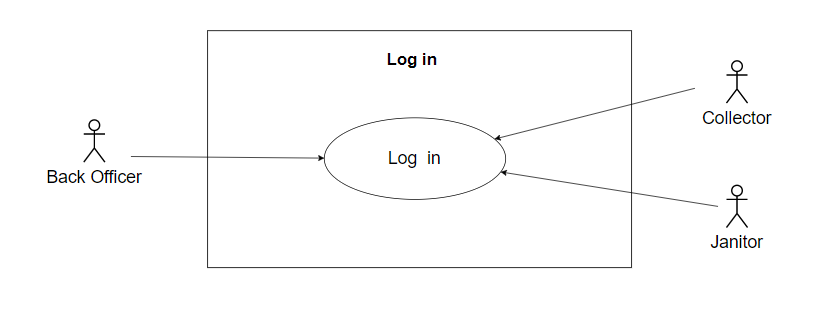
\includegraphics[width=6in]{Image/login.png}
    \end{center}
\end{figure}
\\
\begin{tabular}{|p{3cm}|p{10cm}|}
     \hline
     Use-case name & Log in\\
     \hline
     Actor & Back officer, Collector, Janitor\\
     \hline
     Description & Người dùng muốn đăng nhập vào hệ thống \\
     
     \hline
     Preconditions & Không \\
          \hline
     Postconditions & Người dùng đăng nhập được vào hệ thống \\
     \hline
     Normal flow & 1. Hệ thống cung cấp giao diện để người dùng cung cấp thông tin gồm 2 trường là tài khoản và mật khẩu \\
     & 2. Người dùng nhập thông tin đăng nhập  \\
     & 3. Hệ thống kiểm tra thông tin đăng nhập \\
     & 4. Hệ thống phản hồi người dùng. Nếu tài khoản và mật khẩu đúng thì hệ thống hiện thị giao diện. Nếu sai thì hệ thống sẽ hiển thị thông báo về lỗi sai\\
     \hline
     Exceptions & Người dùng nhập sai hoặc thiếu thông tin đăng nhập\\
     \hline
     Alternative flows & Không\\
     \hline
\end{tabular}
\vspace{0.5cm}

\item \textbf{Tính năng tương tác (Chat)} \\
\begin{figure}[!h]
    \begin{center}
      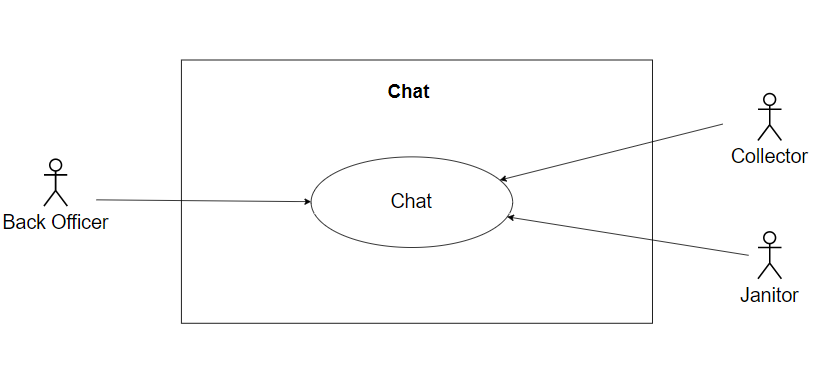
\includegraphics[width=6in]{Image/Chat.png}
    \end{center}
\end{figure}
\\
\textbf{Nhận tin nhắn (Receive message )} \\
\begin{tabular}{|p{3cm}|p{10cm}|}
     \hline
     
     Use-case name & Receive Message \\
     \hline
     Actor & Back officer, Collectors, Janitors\\
     \hline
     Description & Người dùng nhận được tin nhắn gửi tới mình \\
     \hline
     Preconditions & Người dùng phải đăng nhâp vào hệ thống\\
          \hline
     Postconditions & Người dùng nhận được tin nhắn \\
     \hline
     Normal flow & 1. Khi người nào đó gửi tin nhắn tới người dùng, người dùng nhận được thông báo trên góc phải màn hình kèm âm thanh thông báo tin nhắn. \\
     & 2. Người dùng nhấp vào thông báo sẽ chuyển tới hộp thoại nhận tin nhắn và hệ thống sẽ xác nhận tin nhắn đã được đọc \\
     \hline
     Exceptions & Không\\
     \hline
     Alternative flows & Không\\
     \hline
\end{tabular}
\vspace{0.5cm}

\textbf{Gửi tin nhắn (Send message )} \\
\begin{tabular}{|p{3cm}|p{10cm}|}
     \hline
     
     Use-case name & Receive Message \\
     \hline
     Actor & Back officer, Collectors, Janitors\\
     \hline
     Description & Người dùng muốn gửi tin nhắn \\
     \hline
     Preconditions & Người dùng phải đăng nhâp vào hệ thống\\
          \hline
     Postconditions & Người dùng gửi được tin nhắn \\
     \hline
     Normal flow & 1. Người dùng nhập tin nhắn và bấm gửi. Hệ thống sẽ gửi thông báo tới người nhận và đánh đấu nếu gửi thành công \\
     & 2. Riêng Backofficer có khả năng gửi tin nhắn tới nhìều người \\
     \hline
     Exceptions & Không\\
     \hline
     Alternative flows & Không\\
     \hline
\end{tabular}
\vspace{0.5cm}

\item \textbf{Tính năng quản lý công việc (Manage Task)}\\
\begin{figure}[!h]
    \begin{center}
      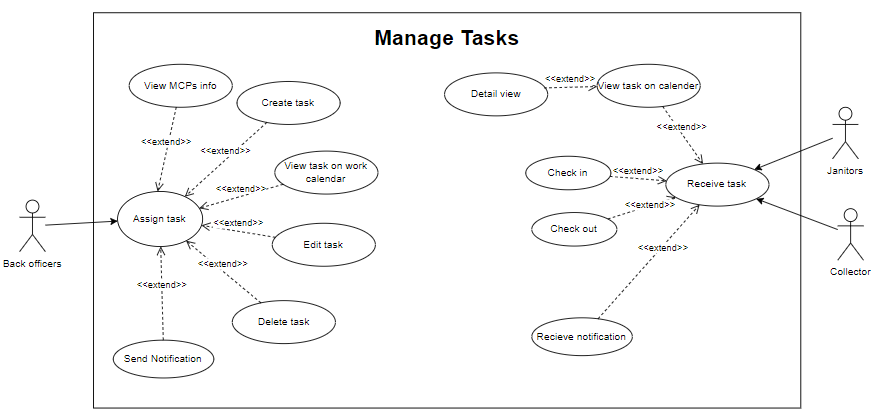
\includegraphics[width=6in]{Image/manage.png}
    \end{center}
\end{figure}
\\

\textbf{Gán công việc (Assign Task)} \\
\begin{tabular}{|p{3cm}|p{10cm}|}
     \hline
     
     Use-case name & Create task \\
     \hline
     Actor & Back officer\\
     \hline
     Description & Back-officer muốn tạo task \\
     \hline
     Preconditions & Người dùng phải đăng nhập vào hệ thống và người dùng phải là Back-officer\\
          \hline
     Postconditions & Back officer tạo công việc thành công cho nhân viên(collectors và janitors) \\
     \hline
     Normal flow & 1. Back-officer tạo công việc dựa trên work-calendar để phân công việc theo thời gian hợp lý. \\
     & 2. Hệ thống sẽ lưu lại công việc vừa tạo trên calendar và thông báo với Back-officer đã tạo thành công, đồng thời gửi thông báo về cho nhân viên tương ứng với công việc vừa tạo. \\
     \hline
     Exceptions & Không\\
     \hline
     Alternative flows & Không\\
     \hline
\end{tabular}
\vspace{0.5cm}

\begin{tabular}{|p{3cm}|p{10cm}|}
     \hline
     Use-case name & Edit task \\
     \hline
     Actor & Back officer\\
     \hline
     Description & Back-officer muốn sửa task đã tạo \\
     \hline
     Preconditions & Người dùng phải đăng nhập vào hệ thống và người dùng phải là Back-officer\\
               \hline
     Postconditions & Back officer sửa thành công task của nhân viên (collectors và janitors)\\
     \hline
     Normal flow & 1. Back-officer sửa công việc dựa trên work-calendar để phân công việc theo thời gian hợp lý. \\
     & 2. Hệ thống sẽ lưu lại công việc vừa sửa trên calendar và thông báo sửa task thành công, đồng thời gửi thông báo về cho nhân viên tương ứng với công việc vừa sửa. \\
     \hline
     Exceptions & Không\\
     \hline
     Alternative flows & Không\\
     \hline
\end{tabular}

\vspace{0.5cm}

\begin{tabular}{|p{3cm}|p{10cm}|}
     \hline
     Use-case name & Delete Task \\
     \hline
     Actor & Back officer, Collector, Janitor\\
     \hline
     Description & Back-officer muốn xóa task đã tạo \\
     \hline
     Preconditions & Người dùng phải đăng nhập vào hệ thống và người dùng phải là Back-officer\\
               \hline
     Postconditions & Người dùng xóa thành công công việc của nhân viên (collectors và janitors) \\
     \hline
     Normal flow & 1. Back-officer xóa công việc trên work calendar. \\
     & 2. Hệ thống sẽ xóa task trên calendar và thông báo nếu xóa task thành công. \\
     \hline
     Exceptions & Không\\
     \hline
     Alternative flows & 1.1. Hệ thống yêu cầu xác nhận chắc chắn muốn xoá task.\\
     & 1.2. Nếu người dùng chọn "Yes" thực hiện bước 2.\\
     & 1.3. Nếu người dùng chọn "No" thì hệ thống không làm gì.\\
     \hline
\end{tabular}
\vspace{0.5cm}\\
\begin{tabular}{|p{3cm}|p{10cm}|}
     \hline
     Use-case name & View Task \\
     \hline
     Actor & Back officer\\
     \hline
     Description & Người dùng quan sát tổng quan lịch làm việc của mình \\
     \hline
     Preconditions & Người dùng phải đăng nhập vào hệ thống.\\
               \hline
     Postconditions & Người dùng có thể đọc tất cả công việc trên work-calendar.\\
     \hline
     Normal flow & 1. Sau các thao tác thêm sửa xóa của Back Officer, end-user có thể view ngắn gọn mình làm việc vào khung giờ nào ở trên work-calendar. \\
     & 2. Người dùng có thể chọn chức năng xem chi tiết (đọc thêm ở bảng view detail) \\
     \hline
     Exceptions & Không\\
     \hline
     Alternative flows & Không\\
     \hline
\end{tabular}




\vspace{0.5cm}

\begin{tabular}{|p{3cm}|p{10cm}|}
     \hline
     Use-case name & View work calendar\\
     \hline
     Actor & Management, Back officer\\
     \hline
     Description & Xem lịch công việc\\
     \hline
     Preconditions & Người dùng phải đăng nhập vào hệ thống và thuộc nhóm Manage hoặc Back oficer\\
     \hline
     Normal flow & 1. Hệ thống hiển thị giao diện lịch các công việc hiện tại.\\
     \hline
     Exceptions & Không\\
     \hline
     Alternative flows & Không.\\
     \hline
\end{tabular}

\vspace{0.5cm}

\textbf{Receive task} \\ \\
 \begin{tabular}{| p{3cm} | p{10cm} |}
  \hline
     Use-case name & View task on calender
     \\
     \hline
     Actor & Collector, Janitor
     \\ \hline
     Description & Collector, Janitor muốn xem thông tin về lịch trình công việc 
      \\
     \hline
     Preconditions & Collector, Janitor đăng nhạp vào hệ thống\\
          \hline
     Postconditions & Collector, Janitor biết được thông tin về công việc của mình
     \\ \hline
      Normal flow & 1. Hệ thống cung cấp các thông tin ngắn gọn về lịch làm việc trên work calendar\\
      & 2. Người dùng có thể chọn chức năng xem chi tiết(đọc thêm ở bảng view detail)
     \\ \hline
     Exceptions & Không 
     \\ \hline
     Alternative flows & Không
     \\ \hline
\end{tabular}\\
\vspace{0.5cm}

 \begin{tabular}{| p{3cm} | p{10cm} |}
  \hline
     Use-case name & Detail view
     \\
     \hline
     Actor & Collector, Janitor
     \\ \hline
     Description & Collector, Janitor muốn xem thông tin chi tiết về lịch trình công việc 
      \\
     \hline
     Preconditions & Collector, Janitor đăng nhạp vào hệ thống\\
          \hline
     Postconditions & Collector, Janitor biết được thông tin chi tiết về công việc của mình
     \\ \hline
      Normal flow & 1. Hệ thống cung cấp các thông tin chi tiết về lịch làm việc bao gồm: ca làm, cộng sự, địa điểm, phương tiện sử dụng\\
      \hline
     Exceptions & Không 
     \\ \hline
     Alternative flows & Không
     \\ \hline
\end{tabular}\\
\vspace{0.5cm}

 \begin{tabular}{| p{3cm} | p{10cm} |}
  \hline
     Use-case name & Check in
     \\
     \hline
     Actor & Collector, Janitor
     \\ \hline
     Description & Collector, Janitor muốn báo cáo tiến độ công việc cho Back oficer
      \\
     \hline
     Preconditions & Collector, Janitor đăng nhạp vào hệ thống\\
          \hline
     Postconditions & Back officer biết được tiến độ công việc của Collector, Janitor
     \\ \hline
      Normal flow & 1. Hệ thống cung cấp giao diện dạng tin nhắn để người dùng soạn thông tin\\

         & 2. Người dùng soạn tin nhắn cần gửi\\
        & 3. Hệ thống gửi tin nhắn đến Back officer \\
        & 4. Nếu tin nhắn gửi thất bại hệ thống sẽ hiển thị thông báo \\
      \hline
     Exceptions & Không 
     \\ \hline
     Alternative flows & Không
     \\ \hline
\end{tabular}\\
\vspace{0.5cm}

 \begin{tabular}{| p{3cm} | p{10cm} |}
  \hline
     Use-case name & Check out
     \\
     \hline
     Actor & Collector, Janitor
     \\ \hline
     Description & Collector, Janitor muốn báo cáo công việc đã hoàn thành  cho Back oficer
      \\
     \hline
     Preconditions & Người dùng đăng nhạp vào hệ thống\\
          \hline
     Postconditions & Back officer biết được các công việc mà Collector, Janitor đã hoàn thành
     \\ \hline
      Normal flow & 1. Hệ thống cung cấp giao diện dạng check box bao gồm các công việc của Collector, Janitor \\

         & 2. Người dùng chọn công việc mà mình đã hoàn thành\\
        & 3. Hệ thống sẽ cập nhật bảng check box của Back officer\\
        & 4. Nếu việc cập nhật bị thất bại hệ thống sẽ hiển thị thông báo \\
      \hline
     Exceptions & Không 
     \\ \hline
     Alternative flows & Không
     \\ \hline
\end{tabular}\\
\vspace{0.5cm}

 \begin{tabular}{| p{3cm} | p{10cm} |}
  \hline
     Use-case name & Recieve notification
     \\
     \hline
     Actor & Collector, Janitor
     \\ \hline
     Description & Collector, Janitor muốn nhận thông báo từ Back officer khi MCP đầy
      \\
     \hline
     Preconditions & Người dùng đăng nhạp vào hệ thống\\
          \hline
     Postconditions & Collector, Janitor xử lý kịp thời khi các MCP đầy
     \\ \hline
      Normal flow & 1. Hệ thống sẽ gửi tin nhắn từ Back officer đến Collector, Janitor về MCP đầy  \\

         & 2.  Collector và Janitor phản hồi tin nhắn với nội dung có thể đến MCP đầy hay không\\
        & 3. Hệ thống sẽ gửi tin nhắn phản hồi đến Back officer\\
    
      \hline
     Exceptions & Không 
     \\ \hline
     Alternative flows & Không
     \\ \hline
\end{tabular}\\
\vspace{0.5cm}


 






\item \textbf{Tính năng quản lý tài khoản(Account management)}
\begin{figure}[!h]
    \begin{center}
      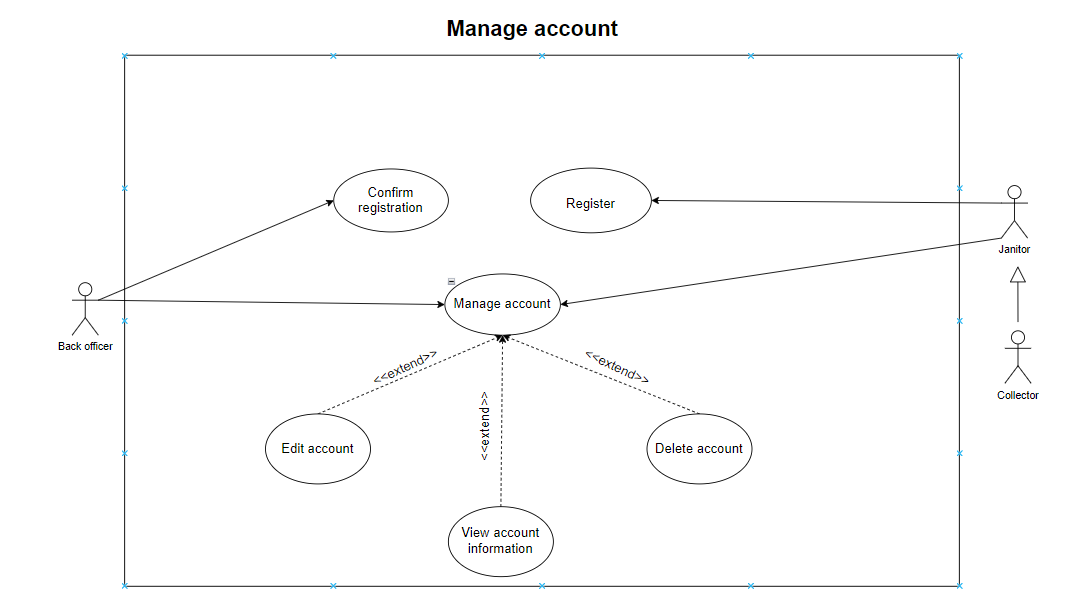
\includegraphics[width=6in]{Image/account.png}
    \end{center}
\end{figure}

\textbf{Register}\\
\begin{tabular}{| p{3cm} | p{10cm} |}
  \hline
     Use-case name & Register
     \\
     \hline
     Actor & Collector, Janitor
     \\ \hline
     Description & Người dùng tạo tài khoản
      \\
     \hline
     Preconditions & Người dùng truy cập vào hệ thống
     \\ \hline
     Post-conditions & Người dùng hoàn thành đăng kí tài khoản
     \\ \hline
      Normal flow & 1.Hệ thống hiển thị giao diện cho người dùng nhập các thông tin cần thiết
      \\
      & 2.Người dùng nhập các thông tin hệ thống yêu cầu  \\

    & 3.Hệ thống xác minh tính hợp lệ của thông tin người dùng cung cấp \\
    & 4.Hệ thống hiển thị thông tin tài khoản cho người dùng \\

    & 5.Hệ thống hiện thị giao diện Account management \\
\hline
     Exceptions & Người dùng nhập thông tin thiếu hoặc không hợp lệ
     \\ \hline
     Alternative flows & Hiện thông báo yêu cầu người dùng nhập lại thông tin
     \\ \hline
     
\end{tabular}\\ 
\vspace{0.5cm} \\
\textbf{Confirm registration}\\
\begin{tabular}{| p{3cm} | p{10cm} |}
  \hline
     Use-case name & Confirm registration
     \\
     \hline
     Actor & Back officer
     \\ \hline
     Description & Người dùng xác nhận đăng ký tài khoản
      \\
     \hline
     Preconditions & Người dùng truy cập vào hệ thống
     \\ \hline
          Post-conditions & Người dùng hoàn thành xác nhận đăng ký
     \\ \hline
      Normal flow & 1.Hệ thống hiển thị giao diện cho người dùng xem các yêu cầu đăng ký mới
      \\
      & 2.Hệ thống hiển thị thông tin đăng kí cho người dùng  \\

    & 3.Người dùng xác nhận thông tin đăng kí\\
    & 4.Hệ thống hiển thị thông tin tài khoản cho người dùng \\

    & 5.Hệ thống hiện thị giao diện Account management \\
\hline
     Exceptions & Không
     \\ \hline
     Alternative flows & Không
     \\ \hline
     
\end{tabular}\\ \\
\vspace{0.5cm} \\
\textbf{Manage account}\\
\begin{tabular}{| p{3cm} | p{10cm} |}
  \hline
     Use-case name & Manage account
     \\
     \hline
     Actor & Back officer, Collector, Janitor
     \\ \hline
     Description & Người dùng quản lý tài khoản
      \\
     \hline
     Preconditions & Người dùng đăng nhập vào hệ thống
     \\ \hline
     Post-conditions & Người dùng hoàn thành quản lý thông tin tài khoản
     \\ \hline
      Normal flow & 1.Hệ thống hiện thỉ giao diện các thông tin người dùng có thể quản lý\\
& 2.Người dùng lựa chọn tác vụ cần quản lý\\
& 3.Hệ thống xác nhận việc quản lý của người dùng\\
& 4.Hệ thống trở về hiển thị giao diện Account management\\
\hline
     Exceptions & Không
     \\ \hline
     Alternative flows & Tại bước 2: Người dùng chọn chỉnh sửa tài khoản thì tiếp tục với use-case "Edit account" \\
     & Người dùng chọn xem thông tin tài khoản thì tiếp tục với use-case "View account information" \\
     & Người dùng chọn xóa tài khoản thì tiếp tục với use-case "Delete account"
     \\ \hline
     
\end{tabular}\\ 
\vspace{0.5cm} \\
\textbf{Edit account} \\
\begin{tabular}{| p{3cm} | p{10cm} |}
  \hline
     Use-case name & Edit account
     \\
     \hline
     Actor & Back officer, Collector, Janitor
     \\ \hline
     Description & Người dùng chỉnh sửa thông tin tài khoản
      \\
     \hline
     Preconditions & Người dùng đăng nhập vào hệ thống
     \\ \hline
           Post-conditions & Thông tin tài khoản được sửa đổi trên hệ thống.
     \\ \hline
      Normal flow & 1.Người dùng chọn chức năng chỉnh sửa thông tin tài khoản \\
      & 2.Hệ thống hiển thị các thông tin người dùng có thể chỉnh sửa \\
      & 3. Người dùng nhấn xác nhận chỉnh sửa\\
& 4.Hệ thống hiện thỉ xác nhận lại yêu cầu của người dùng \\
& 5.Hệ thống chuyển sang giao diện gốc\\
\hline
     Exceptions & Không
     \\ \hline
     Alternative flows & Không
     \\ \hline
     
\end{tabular}\\
\vspace{0.5cm}\\
\textbf{View account information} \\
\begin{tabular}{| p{3cm} | p{10cm} |}
  \hline
     Use-case name & View account information
     \\
     \hline
     Actor & Back officer, Collector, Janitor
     \\ \hline
     Description & Người dùng xem thông tin tài khoản
      \\
     \hline
     Preconditions & Người dùng đăng nhập vào hệ thống
     \\ \hline
           Post-conditions & Người dùng xem được thông tin tài khoản
     \\ \hline
      Normal flow & 1.Người dùng chọn chức năng xem thông tin tài khoản \\
& 2.Hệ thống hiện thỉ thông tin người dùng \\
& 3.Hệ thống trở về giao diện gốc\\
\hline
     Exceptions & Không
     \\ \hline
     Alternative flows & Không
     \\ \hline
     
\end{tabular}\\
\vspace{0.5cm}\\
\textbf{Delete account} \\
\begin{tabular}{| p{3cm} | p{10cm} |}
  \hline
     Use-case name & Delete account
     \\
     \hline
     Actor & Back officer, Collector, Janitor
     \\ \hline
     Description & Người dùng xóa tài khoản
      \\
     \hline
     Preconditions & Người dùng đăng nhập vào hệ thống
     \\ \hline
           Post-conditions & Tài khoản được xóa khỏi hệ thống
     \\ \hline
      Normal flow & 1.Người dùng chọn chức năng xóa tài khoản \\
& 2.Hệ thống hiện thỉ xác nhận lại yêu cầu của người dùng \\
& 3.Hệ thống chuyển sang giao diện gốc\\
\hline
     Exceptions & Không
     \\ \hline
     Alternative flows & Không
     \\ \hline
     
\end{tabular}\\




    \item \textbf{Tính năng manage area}
\\
\begin{figure}[!h]
    \begin{center}
      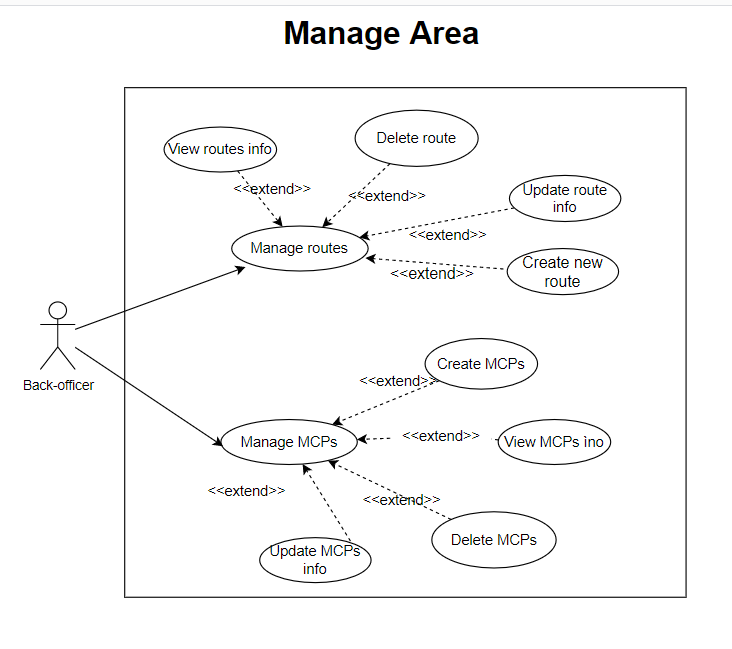
\includegraphics[width=6in]{Image/manageArea_diagram.png}
    \end{center}
\end{figure}
\\
\begin{tabular}{|p{3cm} | p{10cm}|} 
\hline
     Use case name & \textbf{Manage Area}  \\
     \hline
     Actor & Back-officer \\
     \hline
     Description & Back-officer muốn quản lý được thông tin của khu vực cần thu gom rác và tuyến đường thu gom đến MCPs của khu vực đó. \\
     \hline
     Preconditions & Back-officer phải log in vào hệ thống bằng tài khoản được cấp quyền quản lý.\\
     \hline
     Postconditions & Thông tin về khu vực được quản lý dễ dàng. \\
     \hline
     Normal flow & 
     1. Hệ thống hiển thị giao diện cho việc quản lý khu vực và đưa ra 4 option: \\
        & \hspace{1cm} -Quản lý tuyến đường thu gom rác (routes).\\
        & \hspace{1cm} -Quản lý địa điểm thu gom rác (MCPs). \\
    &2. Back-officer lựa chọn một trong hai option. \\
    &3. Hệ thống chuyển sang giao diện một trong hai option. \\
    &4. Back-officer thực hiện quản lý khu vực thu gom rác. \\
    &5. Hệ thống trở về giao diện chính. \\
    \hline 
    Exceptions & Không \\
    \hline
    Alternative flows & Không. \\
\hline
\end{tabular}
\vspace{0.5cm}
\\
 \begin{tabular}{| p{3cm} | p{10cm} |}
  \hline
     Use-case name & \textbf{Manage MCPs}
     \\
     \hline
     Actor & Back-officer
     \\ \hline
     Description & Back-officer muốn quản lý thông tin về địa điểm thu gom rác (MCPs). \\
     \hline
     Preconditions & Back-officer phải log in vào hệ thống bằng tài khoản hợp lệ được cấp quyền quản lý thông tin.
     \\ \hline
     Postconditions & Back-officer quản lý thông tin MCPs thành công. \\
     \hline
      Normal flow & 1. Hệ thống chuyển sang giao diện hiển thị cho việc quản lý MCPs và hiển thị ra 4 option \\
        & \hspace{1cm} -Cập nhật thông tin địa điểm. \\
        & \hspace{1cm} -Xem thông tin địa điểm. \\
        & \hspace{1cm} -Xóa thông tin địa điểm. \\
        & \hspace{1cm} -Thêm thông tin địa điểm. \\ 
    & 2. Back-officer click vào một trong bốn option. \\
    & 3. Hệ thống hiển thị giao diện tương ứng với một trong bốn option. \\
    & 4. Back-officer thực hiện quản lý thông tin của địa điểm thu gom rác. \\
    &5. Hệ thống trở về giao diện chính.\\
\hline
     Exception & Không.  
     \\ \hline
     Alternative flows & Không
     \\ \hline
\end{tabular}
\\
\vspace{0.5cm}  \\
\begin{tabular}{|p{3cm} | p{10cm}|}
\hline
     Use-case name & \textbf{Manage routes}  \\
     \hline
     Actor & Back officer \\
     \hline
     Description & Back officer muốn quản lý thông tin về tuyến đường thu gom rác. \\
     \hline
     Precondition & Back officer phải log in thành công bằng tài khoản được cấp quyền quản lý. \\
    \hline  Postcondition & Back officer thực hiện quản lý thông tin tuyến đường thành công. \\
     \hline 
     Normal flow & 
     1. Hệ thống hiển thị giao diện cho việc quản lý routes và hiện ra 3 option. \\
        &\hspace{1cm} -Xem thông tin tuyến đường. \\
        &\hspace{1cm} -Cập nhật thông tin tuyến đường. \\
        &\hspace{1cm} -Xóa thông tin tuyến đường. \\
     &2. Back officer click chọn một trong ba option. \\
     &3. Hệ thống chuyển sang giao diện một trong ba option tương ứng. \\
     &4. Back officer thực hiện quản lý thông tin tuyến đường. \\
     &5. Hệ thống trở về giao diện chính. \\
    \hline
    Exception & Không. \\
    \hline
    Alternative Flow & Không. \\
\hline
\end{tabular} 
\vspace{0.5cm}
\begin{enumerate}
    \item[c.1)] \textbf{Tính năng manage MCPs} 
    \\ \\ \\
    \begin{tabular}{|p{3cm} | p{10cm}|}
    \hline
         Use-case name & \textbf{Update MCPs)}  \\
         \hline
         Actor & Back officer \\
         \hline 
         Description & Back officer muốn cập nhật thông tin của MCPs trong hệ thống. \\
         \hline
         Preconditions & Back officer phải log in vào hệ thống với tài khoản được cấp quyền quản lý tài nguyên công ty.\\
         \hline
         Normal flow 
         &1. Hệ thống hiển thị thông tin của MCPs (địa chỉ, sức chứa, tình trạng MCPs,...). \\
         &2. Back officer có thể cập nhật các mục thông cần thay đổi của MCPs. \\
         &3. Để xác nhận cập nhật, Back officer click vào nút "Cập nhật thông tin". \\
         &4. Hệ thống hiển thị thông báo "Xác nhận cập nhật thông tin". \\ 
         &5. Nếu Back officer click vào nút "Có", hệ thống sẽ tự động thay đổi những thông tin mới cập nhật. \\
         &6. Hệ thống hiển thị thông báo "Cập nhật thông tin thành công". \\
         &7. Back officer click vào nút "OK". \\
         &8. Hệ thống trở lại giao diện ban đầu. \\
         \hline
    \end{tabular}
    \\ \\ \\
    \begin{tabular}{|p{3cm}|p{10cm}|}
         \hline
         Use-case name & \textbf{Delete MCPs} \\
         \hline
         Actor & Back-officer \\ 
         \hline
         Description & Back-officer muốn xóa thông tin của MCPs ra khỏi hệ thống. \\
         \hline
         Preconditions & Back officer phải log in vào hệ thống bằng tài khoản hợp lệ được cấp quyền quản lý thông tin tài nguyên công ty. \\
         \hline
         Exceptions & Không \\
         \hline
         Normal flows  
         &1. Hệ thống hiển thị danh sách tập các MCPs trong hệ thống. \\
         &2. Back officer chọn ra những MCPs cần xóa thông tin bằng cách click vào checkbox của từng MCPs. \\
         &3.Sau khi chọn xong, Back officer click vào nút "Xóa" ở cuối danh sách. \\
         &4.Hệ thống hiển thị danh sách các MCPs mà Back officer muốn xóa. \\
         &5. Back officer có thể điều chỉnh danh sách xóa bằng cách click vào nút "Xóa" để xóa MCPs ra khởi danh sách xóa.\\
         &6. Để xác nhận xóa thì Back officer click tiếp vào nút "Xóa" bên dưới danh sách MCPs muốn xóa.\\
         &7. Hệ thống hiển thị thông báo "Bạn chắc chắn muốn xóa những MCPs này ra khỏi hệ thống?". \\
         &8. Nếu Back officer click vào nút "Có", hệ thống sẽ tự động xóa thông tin MCPs. \\
         &9. Hệ thống hiển thị thông báo "Xóa thông tin MCPs thành công". \\
         &10. Back officer click vào nút "OK". \\
         &11. Hệ thống trở về giao diện ban đầu. \\
         \hline
         Alternative flow & 
         Alternative Flow 1: tại bước 4: \\
        &1.1 Nếu Back officer không muốn xóa MCPs nữa thì nhấn nút
        "Hủy". \\
        &1.2 Hệ thống trở về giao diện hiển thị danh sách ở bước 3.\\
        &Alternative Flow 2: tại bước 8:\\
        &2.1 Nếu Back officer muốn chỉnh sửa lại danh sách xóa thì click vào nút "Hủy". \\
        &2.2 Hệ thống hiển thị lại danh sách xóa, ở bước 4.\\
        \hline
    \end{tabular}
    \\ \\ \\
    \begin{tabular}{|p{3cm} | p{10cm} |}
    \hline
         Use-case name & \textbf{Create MCPs}  \\
         \hline
         Actor & Back-officer \\
         \hline
         Description & Back-officer muốn thêm thông tin về MCP mới vào hệ thống. \\
         \hline
         Precondition & Back-officer phải log in vào hệ thống bằng tài khoản hợp lệ được cấp quyền quản lý tài nguyên công ty. \\
         \hline 
         Normal flow 
         &1. Hệ thống yêu cầu back-officer phải nhập đầy đủ thông tin của MCPs với đúng định dạng bao gồm: địa chỉ, sức chứa, tình trạng,...\\
         &2. Back-officer phải điền đầy đủ các thông tin bắt buộc với đúng định dạng. \\
         &3. Sau khi điền xong, back-officer click vào nút "Thêm MCPs vào hệ thống". \\
         &4. Hệ thống hiển thị tin nhắn "Bạn có muốn thêm MCPs này vào hệ thống?". \\
         &5. Back officer click vào nút "Có" để xác nhận thêm.\\
         &6. Hệ thống hiển thị thông báo "Thêm MCPs thành công vào hệ thống". \\
         &7. Back-officer click vào nút OK. \\
         &8. Hệ thống trở về giao diện ban đầu.\\
         \hline
         Alternative flow & 
         Alternative flow 1: tại bước 5: \\
         &5.1 Nếu back-officer không muốn thêm MCPs mới vào hệ thống nữa thì chọn nút "Hủy". \\
         &5.2 Hệ thống trở về giao diện điền thông tin của MCPs mới. \\
         \hline
    \end{tabular}
    \\ \\ \\
    \begin{tabular}{|p{3cm} |p{10cm} |}
         \hline
         Use-case name & \textbf{View MCPs info}  \\
         \hline 
         Actor & Back officer \\
         \hline
         Description & Back officer muốn xem thông tin chi tiết của địa điểm thu gom rác trong hệ thống. \\
         \hline
         Preconditions & Back officer phải log in vào hệ thống bằng tài khoản hợp lệ được cấp quyền quản lý thông tin. \\
         \hline
         Normal flow & 
         1. Hệ thống hiển thị thông tin chi tiết của địa điểm thu gom rác (địa chỉ, hình ảnh, sức chứa, tình trạng hiện tại...). \\
         &2. Sau khi xem xong, Back officer click nút "Hoàn thành xem" để trở lại giao diện chính. \\
         \hline
         Exceptions & Không. \\
         \hline
         Alternative flow & Không. \\
         \hline
    \end{tabular}
    \\ \\ \\
    \item[c.2)] \textbf{Tính năng manage routes}.
    \\ \\ \\
    \begin{tabular}{|p{3cm} | p{10cm}|}
    \hline
         Use-case name & \textbf{Update routes)}  \\
         \hline
         Actor & Back-officer \\
         \hline 
         Description & Back-officer muốn cập nhật thông tin của tuyến đường thu gom rác trong hệ thống. \\
         \hline
         Preconditions & Back-officer phải log in vào hệ thống với tài khoản được cấp quyền quản lý thông tin.\\
         \hline
         Normal flow 
         &1. Hệ thống hiển thị thông tin của tuyến đường (tên, lộ trình, chiều dài đường đi, thời gian...). \\
         &2. Back-officer có thể cập nhật các mục thông cần thay đổi của đường đi. \\
         &3. Để xác nhận cập nhật, Back officer click vào nút "Cập nhật thông tin". \\
         &4. Hệ thống hiển thị thông báo "Xác nhận cập nhật thông tin". \\ 
         &5. Nếu Back officer click vào nút "Có", hệ thống sẽ tự động thay đổi những thông tin mới cập nhật. \\
         &6. Hệ thống hiển thị thông báo "Cập nhật thông tin thành công". \\
         &7. Back-officer click vào nút "OK". \\
         &8. Hệ thống trở lại giao diện ban đầu. \\
         \hline
        Exception & Exception 1. \\
        &1.1. Nếu back-officer không nhập đầy đủ thông tin tại những mục bắt buộc thì hệ thống hiển thị thống báo "Hãy nhập đầy đủ thông tin đường ". \\
        &1.2 Back-officer phải nhập đầy đủ thông của nhân viên. \\
        &Exception 2.\\
        &2.1 Nếu back-officer không nhập đúng định dạng thông tin thì hệ thống hiển thị "Hãy nhập đúng định dang: [kiểu định dang]".\\
        &2.2 Back-officer phải nhập đúng định dạng thông tin.\\
        \hline
        Alternative flow & Alternative flow 1: tại bước 3 \\
        &3.1 Nếu back-officer nhập sai thông tin cần chỉnh sửa và muốn thay đổi lại thì click vào nút "Khôi phục thông tin cũ của đường đi". \\
        &3.2 Hệ thống khôi phục lại thông tin cũ trước khi nhập. \\
        &Alternative flow 2: tại bước 5 \\
        &5.1 Nếu back-officer không muốn cập nhật thông tin của đường đi nữa thì click vào nút "Hủy". \\
        &5.2 Hệ thống trở về giao diện chỉnh sửa như bước 2.\\
        \hline
    \end{tabular}
    \\ \\ \\
    \begin{tabular}{|p{3cm}|p{10cm}|}
         \hline
         Use-case name & \textbf{Delete route} \\
         \hline
         Actor & Back-officer \\ 
         \hline
         Description & Back-officer muốn xóa thông tin của tuyến đường thu gom rác ra khỏi hệ thống. \\
         \hline
         Preconditions & Back-officer phải log in vào hệ thống bằng tài khoản hợp lệ được cấp quyền quản lý. \\
         \hline
         Postconditions & Back-officer xóa thành công thông tin của tuyến đường ra khỏi hệ thống. \\
         \hline
         Normal flows  
         &1. Hệ thống hiển thị danh sách tập các MCPs trong hệ thống. \\
         &2. Back officer chọn ra những tuyến đường cần xóa thông tin bằng cách click vào checkbox của từng tuyến đường. \\
         &3.Sau khi chọn xong, Back officer click vào nút "Xóa" ở cuối danh sách. \\
         &4.Hệ thống hiển thị danh sách các tuyến đường mà back-officer muốn xóa. \\
         &5. Back officer có thể điều chỉnh danh sách xóa bằng cách click vào nút "Xóa" để xóa tuyến đường ra khởi danh sách xóa.\\
         &6. Để xác nhận xóa thì Back officer click tiếp vào nút "Xóa" bên dưới danh sách tuyến đường muốn xóa.\\
         &7. Hệ thống hiển thị thông báo "Bạn chắc chắn muốn xóa những tuyến đường này ra khỏi hệ thống?". \\
         &8. Nếu Back officer click vào nút "Có", hệ thống sẽ tự động xóa thông tin tuyến đường. \\
         &9. Hệ thống hiển thị thông báo "Xóa thông tin tuyến đường thành công". \\
         &10. Back officer click vào nút "OK". \\
         &11. Hệ thống trở về giao diện ban đầu. \\
         \hline
         Alternative flow & 
         Alternative Flow 1: tại bước 4: \\
        &4.1 Nếu Back officer không muốn xóa MCPs nữa thì nhấn nút
        "Hủy". \\
        &4.2 Hệ thống trở về giao diện hiển thị danh sách ở bước 3.\\
        &Alternative Flow 2: tại bước 8:\\
        &8.1 Nếu Back officer muốn chỉnh sửa lại danh sách xóa thì click vào nút "Hủy". \\
        &8.2 Hệ thống hiển thị lại danh sách xóa, ở bước 4.\\
        \hline
    \end{tabular}
    \\ \\ \\
    \begin{tabular}{|p{3cm} | p{10cm} |}
    \hline
         Use-case name & \textbf{Create new route}  \\
         \hline
         Actor & Back-officer \\
         \hline
         Description & Back-officer muốn thêm thông tin về tuyến đường thu gom rác mới vào hệ thống. \\
         \hline
         Precondition & Back-officer phải log in vào hệ thống bằng tài khoản hợp lệ được cấp quyền quản lý. \\
         \hline 
         Postcondition & Back-officer thêm thông tin về tuyến đường thu gom rác mới vào hệ thống thành công. \\
         \hline
         Normal flow 
         &1. Hệ thống yêu cầu back-officer phải nhập đầy đủ thông tin của tuyến đường với đúng định dạng bao gồm: tên đường đi, chiều dài, thời gian hoạt động, ...\\
         &2. Back-officer phải điền đầy đủ các thông tin bắt buộc với đúng định dạng. \\
         &3. Sau khi điền xong, back-officer click vào nút "Thêm tuyến đường vào hệ thống". \\
         &4. Hệ thống hiển thị tin nhắn "Bạn có muốn thêm tuyến đường này vào hệ thống?". \\
         &5. Back officer click vào nút "Có" để xác nhận thêm.\\
         &6. Hệ thống hiển thị thông báo "Thêm tuyến đường thành công vào hệ thống". \\
         &7. Back-officer click vào nút OK. \\
         &8. Hệ thống trở về giao diện ban đầu.\\
         \hline
         Alternative flow & 
         Alternative flow 1: tại bước 5: \\
         &5.1 Nếu back-officer không muốn thêm tuyến đường mới vào hệ thống nữa thì chọn nút "Hủy". \\
         &5.2 Hệ thống trở về giao diện điền thông tin của tuyến đường mới. \\
         \hline
    \end{tabular}
    \\ \\ \\
    \begin{tabular}{|p{3cm} |p{10cm} |}
         \hline
         Use-case name & \textbf{View routes info}  \\
         \hline 
         Actor & Back-officer \\
         \hline
         Description & Back-officer muốn xem thông tin chi tiết của tuyến đường thu gom rác trong hệ thống. \\
         \hline
         Preconditions & Back-officer phải log in vào hệ thống bằng tài khoản hợp lệ được cấp quyền quản lý thông tin. \\
         \hline
         Normal flow & 
         1. Hệ thống hiển thị thông tin chi tiết của tuyến đường thu gom rác (lộ trình, chiều dài dường đi, thời gian,...). \\
         &2. Sau khi xem xong, Back officer click nút "Hoàn thành xem" để trở lại giao diện chính. \\
         \hline
         Exceptions & Không. \\
         \hline
         Alternative flow & Không. \\
         \hline
    \end{tabular}
    \newpage
    \item[c.3)] \textbf{Tính năng manage vehicle and troller}
    \\
    \begin{figure}[!h]
        \centering
        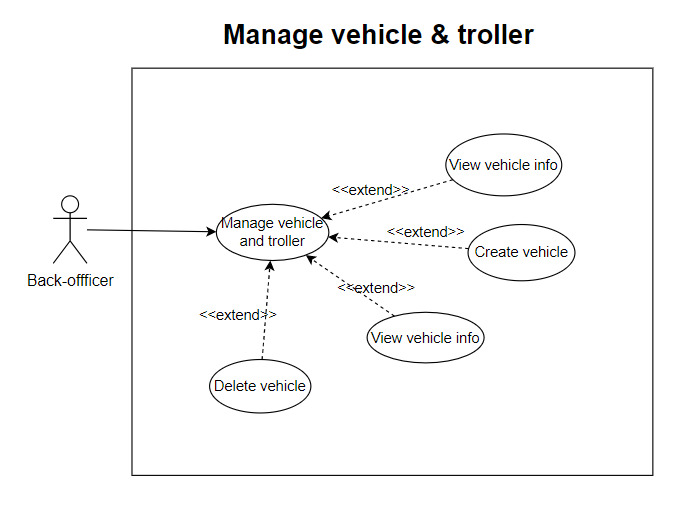
\includegraphics[width=6in]{Image/manageVehicle_diagram.png}
    \end{figure}
    \\
    \begin{tabular}{| p{3cm} | p{10cm} |}
    \hline
         Use-case name & \textbf{Manage Vehicle}  \\
         \hline
         Actor & Back-officer \\
         \hline 
         Description & Back-officer muốn quản lý thông tin tài nguyên về xe rác và thùng rác trong hệ thống. \\
         \hline 
         Preconditions & Back-officer phải log in vào hệ thống với tài khoản được cấp quyền quản lý. \\
         \hline
         Normal flow 
         &1. Hệ thống hiển thị giao diện gồm 4 option để quản lý thông tin vehicle: \\
            &\hspace{1cm} -Xóa xe rác (thùng rác) ra khỏi hệ thống. \\
            &\hspace{1cm} -Thêm xe rác (thùng rác)  vào hệ thống. \\
            &\hspace{1cm} -Xem thông tin xe rác (thùng rác). \\
            &\hspace{1cm} -Cập nhật thông tin xe rác (thùng rác). \\
        &2. Back-officer click vào 1 trong 4 option. \\
        &3. Hệ thống chuyển sang giao diện của 1 trong 4 option vừa chọn. \\
        &4. Back-officer thực hiện xong công việc quản lý thông tin. \\
        &5. Hệ thống trở về giao diện chính.\\
        \hline
        Exception & Không \\
        \hline
        Alternative flow & Không \\
        \hline
    \end{tabular}
    \\ \\ \\
    \begin{tabular}{|p{3cm} | p{10cm}|}
    \hline
         Use-case name & \textbf{Update vehicle info}  \\
         \hline
         Actor & Back officer \\
         \hline 
         Description & Back officer muốn cập nhật thông tin của xe rác (thùng rác) trong hệ thống. \\
         \hline
         Preconditions & Back officer phải log in vào hệ thống với tài khoản được cấp quyền quản lý.\\
         \hline
         Normal flow 
         &1. Hệ thống hiển thị thông tin của vehicle (số xe, tải trọng, loại xe,...). \\
         &2. Back officer có thể cập nhật các mục thông cần thay đổi của vehicle. \\
         &3. Để xác nhận cập nhật, back officer click vào nút "Cập nhật thông tin". \\
         &4. Hệ thống hiển thị thông báo "Xác nhận cập nhật thông tin". \\ 
         &5. Nếu Back officer click vào nút "Có", hệ thống sẽ tự động thay đổi những thông tin mới cập nhật. \\
         &6. Hệ thống hiển thị thông báo "Cập nhật thông tin thành công". \\
         &7. Back officer click vào nút "OK". \\
         &8. Hệ thống trở lại giao diện ban đầu. \\
         \hline
    \end{tabular}
    \\ \\ \\
    \begin{tabular}{|p{3cm} |p{10cm} |}
         \hline
         Use-case name & \textbf{View routes info}  \\
         \hline 
         Actor & Back-officer \\
         \hline
         Description & Back-officer muốn xem thông tin chi tiết của tuyến đường thu gom rác trong hệ thống. \\
         \hline
         Preconditions & Back-officer phải log in vào hệ thống bằng tài khoản hợp lệ được cấp quyền quản lý thông tin. \\
         \hline
         Normal flow & 
         1. Hệ thống hiển thị thông tin chi tiết của tuyến đường thu gom rác (lộ trình, chiều dài dường đi, thời gian,...). \\
         &2. Sau khi xem xong, Back officer click nút "Hoàn thành xem" để trở lại giao diện chính. \\
         \hline
         Exceptions & Không. \\
         \hline
         Alternative flow & Không. \\
         \hline
    \end{tabular}
    \\ \\ \\
    \begin{tabular}{|p{3cm}|p{10cm}|}
         \hline
         Use-case name & \textbf{Delete vehicle} \\
         \hline
         Actor & Back officerr \\ 
         \hline
         Description & Back officer muốn xóa thông tin của xe rác (thùng rác) ra khỏi hệ thống. \\
         \hline
         Preconditions & Back officer phải log in vào hệ thống bằng tài khoản hợp lệ được cấp quyền quản lý thông tin tài nguyên công ty. \\
         \hline
         Exceptions & Không \\
         \hline
         Normal flows  
         &1. Hệ thống hiển thị danh sách tập các xe rác (thùng rác) trong hệ thống. \\
         &2. Back officer chọn ra những vehicle cần xóa thông tin bằng cách click vào checkbox của từng phương. \\
         &3.Sau khi chọn xong, back officer click vào nút "Xóa" ở cuối danh sách. \\
         &4.Hệ thống hiển thị danh sách các vehicle mà back-officer muốn xóa. \\
         &5. Back-officer có thể điều chỉnh danh sách xóa bằng cách click vào nút "Xóa" để xóa vehicle ra khởi danh sách xóa.\\
         &6. Để xác nhận xóa thì Back officer click tiếp vào nút "Xóa" bên dưới danh sách vehicle muốn xóa.\\
         &7. Hệ thống hiển thị thông báo "Bạn chắc chắn muốn xóa những vehicle này ra khỏi hệ thống?". \\
         &8. Nếu Back-officer click vào nút "Có", hệ thống sẽ tự động xóa thông tin vehicle. \\
         &9. Hệ thống hiển thị thông báo "Xóa thông tin phương tiện thành công". \\
         &10. Back-officer click vào nút "OK". \\
         &11. Hệ thống trở về giao diện ban đầu. \\
         \hline
         Alternative flow & 
         Alternative Flow 1: tại bước 4: \\
        &1.1 Nếu Back-officer không muốn xóa vehicle nữa thì nhấn nút
        "Hủy". \\
        &1.2 Hệ thống trở về giao diện hiển thị danh sách ở bước 3.\\
        &Alternative Flow 2: tại bước 8:\\
        &2.1 Nếu back-officer muốn chỉnh sửa lại danh sách xóa thì click vào nút "Hủy". \\
        &2.2 Hệ thống hiển thị lại danh sách xóa, ở bước 4.\\
        \hline
    \end{tabular}
    \\ \\ \\
    \begin{tabular}{|p{3cm} | p{10cm} |}
    \hline
         Use-case name & \textbf{Create vehicle}  \\
         \hline
         Actor & Y's Back officer \\
         \hline
         Description & Back officer muốn thêm thông tin về MCP mới vào hệ thống. \\
         \hline
         Precondition & Back officer phải log in vào hệ thống bằng tài khoản hợp lệ được cấp quyền quản lý tài nguyên công ty. \\
         \hline 
         Normal flow 
         &1. Hệ thống yêu cầu Back officer phải nhập đầy đủ thông tin của vehicle với đúng định dạng bao gồm: số xe, loại xe, tải trọng,...\\
         &2. Back officer phải điền đầy đủ các thông tin bắt buộc với đúng định dạng. \\
         &3. Sau khi điền xong, Back officer click vào nút "Thêm vehicle vào hệ thống". \\
         &4. Hệ thống hiển thị tin nhắn "Bạn có muốn thêm vehicle này vào hệ thống?". \\
         &5. Back officer click vào nút "Có" để xác nhận thêm.\\
         &6. Hệ thống hiển thị thông báo "Thêm vehicle thành công vào hệ thống". \\
         &7. Back officer click vào nút OK. \\
         &8. Hệ thống trở về giao diện ban đầu.\\
         \hline
         Alternative flow & 
         Alternative flow 1: tại bước 5: \\
         &1.1 Nếu Back officer không muốn thêm vehicle vào hệ thống nữa thì chọn nút "Hủy". \\
         &1.2 Hệ thống trở về giao diện điền thông tin của vehicle mới. \\
         \hline
    \end{tabular}
\end{enumerate}

\end{enumerate}
\section{Task 2:  System modelling}

\subsection{Draw an activity diagram to capture the business process between systems and the stakeholders in Task Assignment module}
\newpage
\begin{figure}[!h]
    \begin{center}
      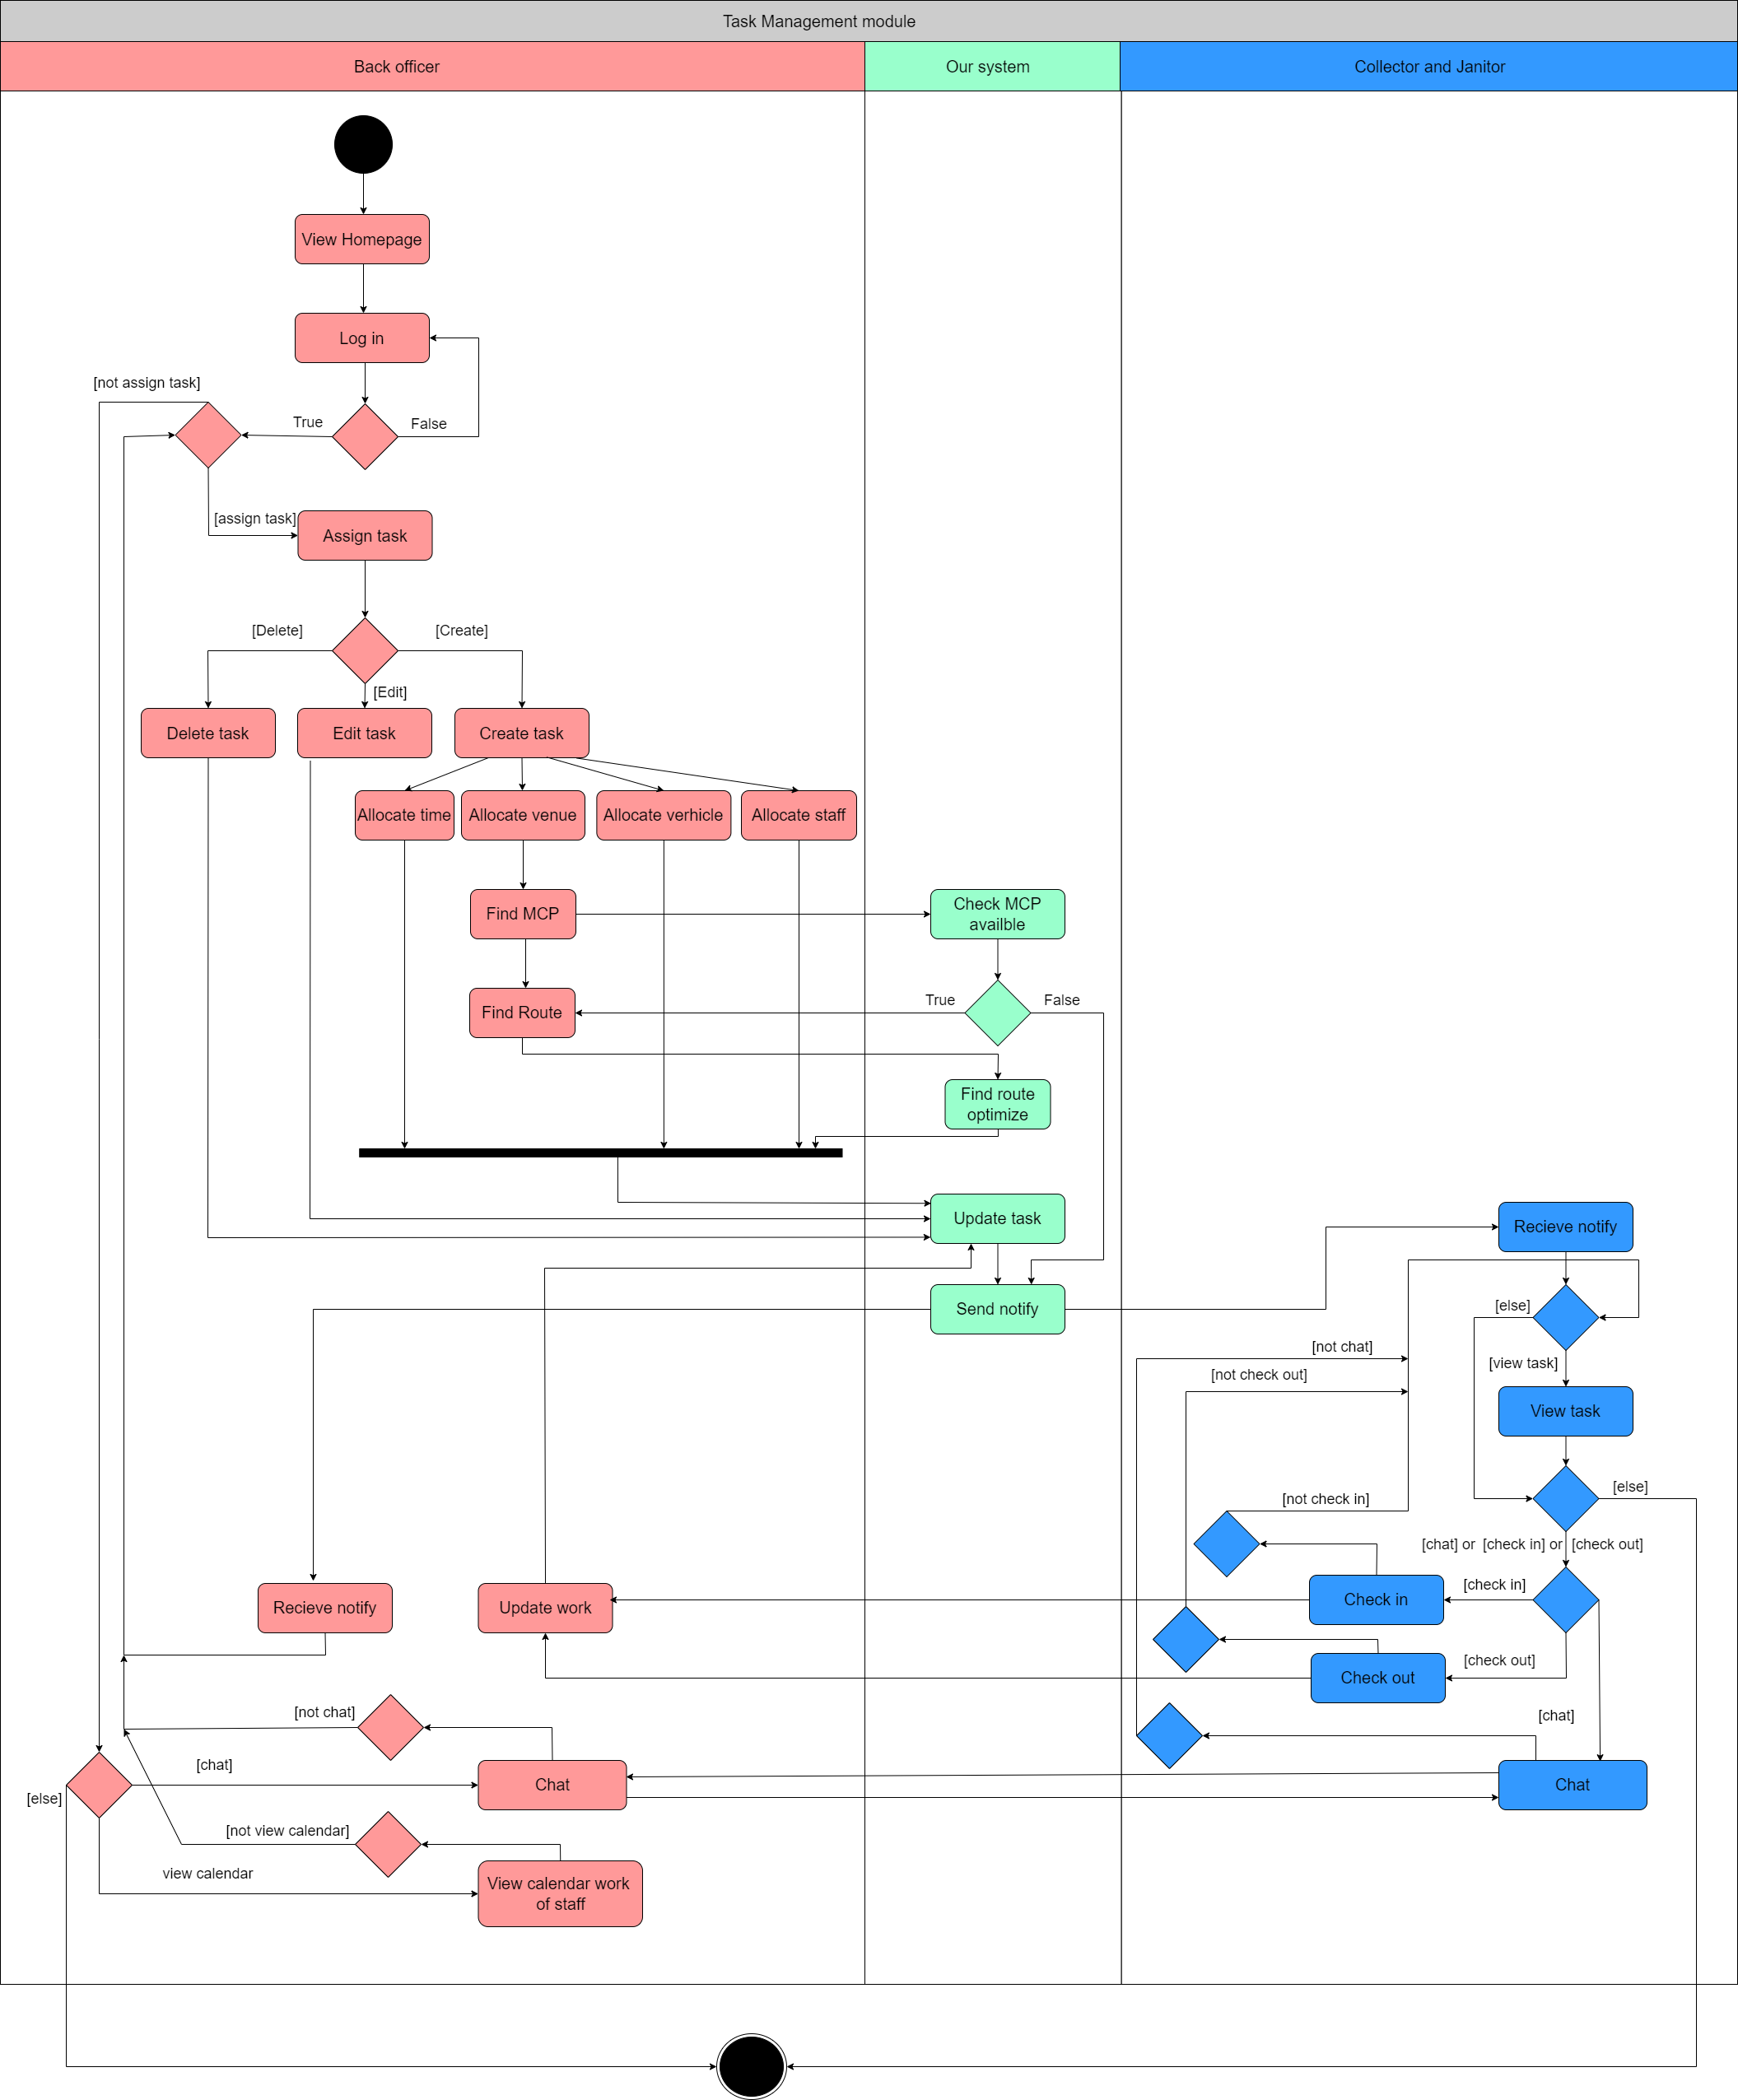
\includegraphics[width=6in]{Image/activity_diagram.png}
    \end{center}
\end{figure}

Link diagram: \url{https://app.diagrams.net/#G18ej9PUIOD8sJmzp6tkr3NTYe7TG1CP-M}
\vspace{0.5cm}
\\
\textbf{Mô tả}\\
Ta chọn start point là ở góc nhìn của \textbf{Back Officer}
\begin{itemize}
    \item Người sau khi truy cập vào ứng dụng sẽ phải đăng nhập để sử dụng ứng dụng.
    \item Ở bước đăng nhập (Log in), nếu người dùng nhập đúng thông tin được lưu trong hệ thống, người dùng sẽ tùy chọn các tính năng: \textit{Assign task}, \textit{Chat} và \textit{View Calendar}.
    \item Tiếp theo, nếu người dùng chọn chức năng \textit{Assign task} - giao nhiệm vụ, sẽ có 3 lựa chọn:
    \begin{itemize}
        \item \textit{Create task} - tạo task mới, chức năng này bao gồm gán yêu cầu thời gian (allocate time), gán địa điểm (venue), phương tiện (vehicle), nhân viên (staff). 
        \item[] Ở tính năng gán địa điểm (allocate venue), yêu cầu hệ thống tính toán, tìm được các MCPs cần thu gom, và từ đó tìm ra đường đi tối ưu để giảm thiểu chi phí.
        \item[] Nếu hệ thống tìm được availble MCPs $\rightarrow$ tìm ra đường đi tối ưu. Nếu không có MCPs nào, thì hệ thống gửi thông báo về cho \textbf{Back Officer} và trở về trang chủ.
        \item \textit{Create task} - sửa task (thay đổi người thực hiện, thay đổi vị trí của MCPs,....)
        \item \textit{Delete task} - xóa task
    \end{itemize}
        \item[] Ở cả 3 tùy chọn trên, nếu thực hiện thành công, hệ thống sẽ tự động update task, calendar. Và gửi thông báo về cho những người lên quan (Back officer, collector và janitor). Sau đó, hệ thống sẽ đưa người dùng trở về trang chủ. Người dùng có thể tiếp tục lựa chọn các tính năng khác như \textit{Chat, View Calendar} hoặc rời đi.
    \item \textit{Chat} - người dùng vào tính năng này để giao tiếp bằng tin nhắn.
    \item \textit{View Calendar} - người dùng xem lịch làm việc của mình (đối với Janitor, Collector) và xem lịch làm việc của nhân viên (Back Officer).
\end{itemize}
    Đối với \textbf{Janitor} và \textbf{Collector}, sau khi được \textit{Assign task}, họ sẽ nhận được thông báo và họ có thể xem sau khi đã đăng nhập vào hệ thống. Từ đó, người dùng có các lựa chọn:
    \begin{itemize}
        \item Họ có thể xem task mà mình đã được phân công từ bảng thông báo.
        \item Thực hiện lựa chọn các tính năng khác như \textit{Chat, Check in, Check out}
        \item Hoặc thoát khỏi chương trình.
    \end{itemize}
    $\rightarrow$ Từ bảng thông báo, người dùng cũng có thể vào tính năng \textit{Check in, Check out} để thực hiện Check in hoặc Check out công việc đã được phân công.\\
    $\rightarrow$  Nếu \textit{Check in, Check out} thành công, hệ thống sẽ update tình trạng của task tự động $\rightarrow$ từ đó update calendar.

\subsection{Proposal a conceptual solution for the route planning task and draw a sequence diagram to illustrate it}
\newpage
\begin{figure}[!h]
    \begin{center}
      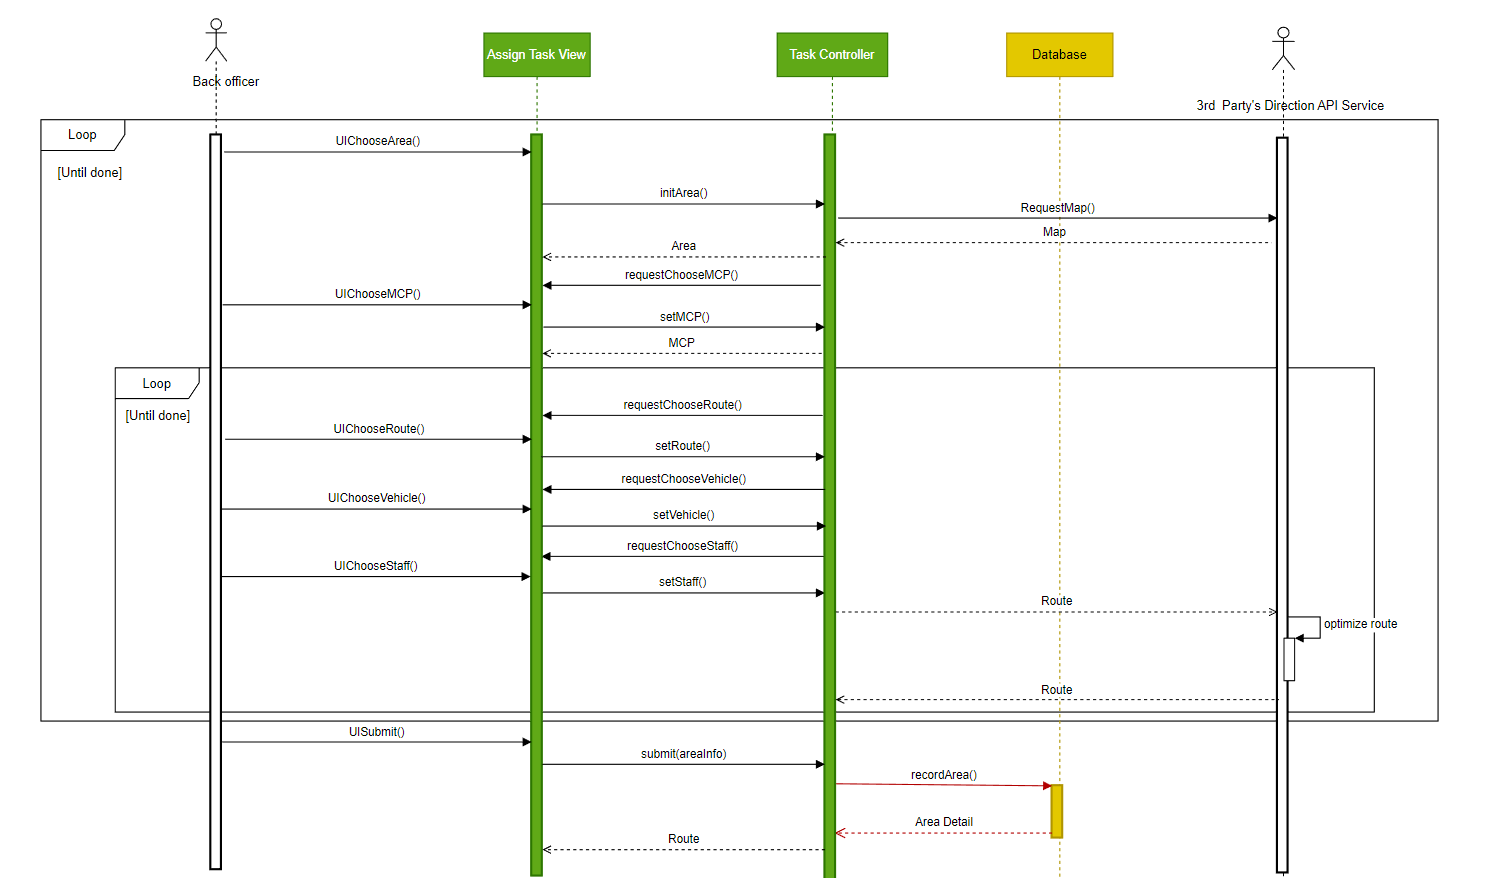
\includegraphics[width=\textwidth]{Image/sdRoute.png}
    \end{center}
\end{figure}
\textbf{Mô tả:}
\begin{itemize}
    \item Một khu vực sẽ bao gồm các thông tin: địa điểm khu vực công việc, các vị trí MCP trong khu vực, các tuyến đường (được tối ưu thông qua hệ thống thứ ba), danh sách nhân viên tham gia công việc.
    \item Người dùng chọn khu vực xác định công việc thông qua bản đồ điện tử của bên thứ ba cung cấp. Khi đó hệ thống khởi tạo một khu vực rỗng thông tin và yêu cầu người dùng chọn một MCP (Major Collecting Point).
    \item Người dùng chọn điểm MCP thông qua bản đồ điện tử. Hệ thống sẽ cập nhật thông tin MCP, sau đó yêu cầu các thông tin về tuyến đường, các phương tiện vận chuyển và các nhân viên tham gia vào công việc. Sau đó hệ thống sẽ gửi thông tin toạ độ của các MCP qua hệ thống thứ ba để tính toán tối ưu đường đi.
    \item Hệ thống thứ ba gửi thông tin tuyến đường đã tối ưu về cho hệ thống quản lý công việc. Hệ thống sẽ cập nhật thông tin tuyến đường của khu vực đã chọn. Việc chọn tuyến đường được lặp lại đến khi xong.
    \item Sau cùng, người dùng thông qua giao diện submit, bấm nút submit. Thông tin chi tiết của area sẽ lưu vào database ở phía server và gửi các message tương ứng.
\end{itemize}
\subsection{Draw a class diagram of Task Assignment module as comprehensive as possible}
\newpage
\begin{figure}[!h]
    \begin{center}
      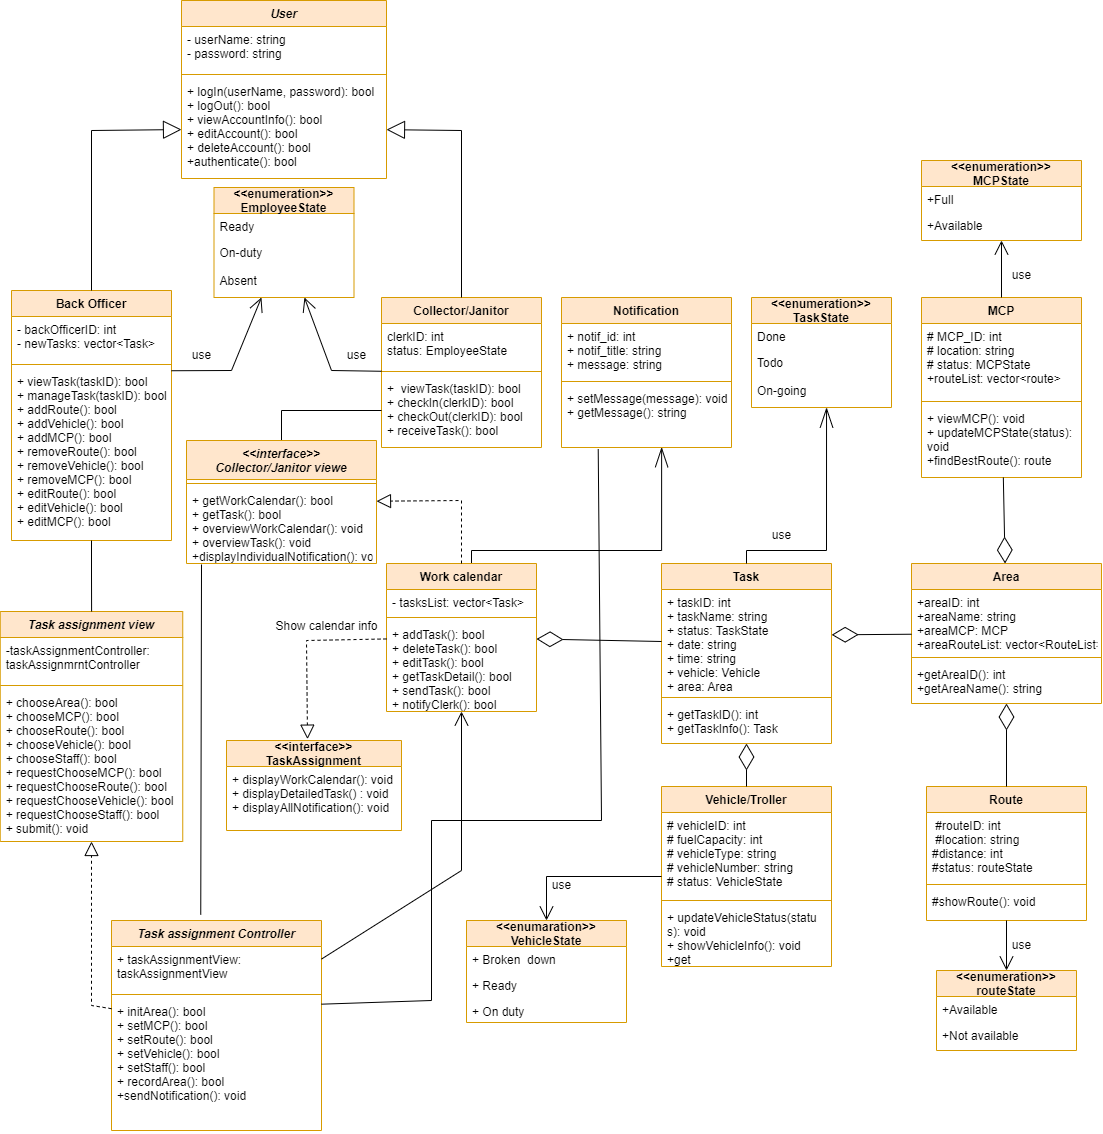
\includegraphics[width=6in]{Image/TaskAssignmentClass.drawio.png}
    \end{center}
\end{figure} 
\\
Link diagram: \url{https://drive.google.com/file/d/16tQafKOAQ0X4cEHqD2Em772F_R33cF9d/view?usp=sharing}
\\
\newpage
\textbf{Mô tả:}
\begin{itemize}
    \item Giao diện chính của UWC2.0 có trang đăng nhập. \textbf{Backofficer},  \textbf{collector} và  \textbf{janitor} đã đăng kí sẽ có \textit{userName} và \textit{password}, và một vài method khác như: logIn, logOut,...
     \textit{userName} và \textit{password} tương ứng. Sau khi người dùng nhập thông tin, thông tin sẽ được gửi đến \textbf{Server},
    \item \textbf{Lịch làm việc} (\textit{work calendar}) sẽ lưu trữ danh sách các công việc (\textit{task}) được tạo ra và đưa lên bởi \textbf{Back officer}. Khi người dùng muốn thao tác với các công việc sẽ chuyển sang giao diện của lịch làm việc.
    \item \textbf{Back officer} có thể tạo ra công việc mới trên lịch làm việc, sau khi công việc được tạo được đưa lên lịch làm việc.
    Thông tin công việc đưa lên lịch làm việc sẽ lưu các thông tin như \textit{mã số công việc}, \textit{thời gian}, \textit{ngày}, \textit{tháng}. Ngoài ra, nội dung chi tiết của công việc lưu các thông tin chi tiết về \textit{
phương tiện}, \textit{tuyến đường} cần làm việc và \textit{các điểm thu gom chính} (MCPs). Lúc này, công việc mới đưa lên lịch làm việc sẽ ở trạng thái To do. Trong các công việc, \textbf{Back officer} có thể quản lý các thông tin về \textit{
phương tiện}, \textit{tuyến đường} cần làm việc và \textit{các điểm thu gom chính}.
    \begin{itemize}
        \item \textbf{Back officer} có thể tạo mới, xóa, sửa thông tin về \textit{tuyến đường} (route). Các thông tin về tuyến đường như \textit{mã số}, \textit{địa điểm}, và \textit{quãng đường}.
        \item \textbf{Back officer} có thể tạo mới, xóa, sửa thông tin về các điểm \textit{thu thập chính} (MCPs). Các thông tin về điểm thu thập như \textit{mã số}, \textit{địa điểm}, và \textit{trạng thái}. Các trạng thái của \textit{điểm thu thập} có thể là đầy hay trống. Trạng thái sẽ được cập nhật sau khi hoàn thành các công việc.
        \item \textbf{Back officer} có thể tạo mới, xóa, sửa thông tin về các \textit{phương tiện} (Vehicle). Các thông tin về phương tiện như \textit{mã số phương tiện}, \textit{tên phương tiện}, \textit{số hiệu phương tiện}, \textit{tình trạng nhiên liệu} và \textit{trạng thái của phương tiện}. Khi phương tiện thuộc công việc được nhận, sẽ chuyển sang trạng thái \textit{On duty}, khi không được sử dụng phương tiện sẽ ở trạng thái \textit{Ready}. Đối với các phương tiện đang được sửa chữa sẽ ở trạng thái \textit{Broken down}.
        \item Các thao tác mà back-officer có thể thực hiện trên Task assignment View như: chọn địa điểm (choose Area), chọn nhân viên (Choose employee) sẽ được Task assignmet controller thao tác trực tiếp với dữ liệu trên Work Calendar với những hàm như: thay đổi MCP (set MCP),... Đồng thời, mỗi khi một task được tạo ra trên Work Calendar, hệ thống tự động tạo ra 1 notification cho back-officer thông qua Task Assignemnt Controller và hiển thị một thông báo trên Task Assignment View.
    \end{itemize}
    \item Janitor/Collector cũng tương tác với Work Calendar qua interface Janitor/Collector. Qua đó, mọi thông tin về task dều được hiển thị lên trang lịch trình riêng của mỗi Janitor/Collect. Đồng thời, Khi có công việc mới được đưa lên bởi back-officer, lịch làm việc sẽ tạo ra \textit{thông báo} với nội dung chi tiết về việc công việc, sau đó gửi thông báo cho \textbf{collector/janitor}, khi có thông tin thay đổi về chi tiết công việc đến từ \textbf{Back officer}, \textbf{collector/janitor} sẽ nhận được chi tiết về thay đổi đó trên lịch làm việc.
    \item Mỗi ngày, \textbf{collector/janitor} vào lịch làm việc để điểm danh và nhận công việc, sau khi nhận công việc, trạng thái của công việc sẽ chuyển sang \textit{On-going}.
    \item Khi nhận công việc, \textbf{collector/janitor} sẽ được chuyển sang giao diện thông tin chi tiết công việc. Tại đây, \textbf{collector/janitor}  có thể quan sát thông tin chi tiết về \textit{tuyến đường}, \textit{điểm thu thập chính} và \textit{phương tiện} mà họ sử dụng. Khi bắt đầu công việc, \textit{phương tiện} được sử dụng trong công việc sẽ chuyển sang trạng thái \textit{On duty} và về lại trạng thái \textit{Ready} sau khi hoàn thành.  Khi kết thúc công việc, điểm thu thập chính trong công việc sẽ chuyển sang trạng thái \textit{Available}.
    \item  Vào cuối ngày, sau khi hoàn thành công việc, \textbf{collector/janitor} thực hiện \textit{check out} trên lịch làm việc, khi đó, trạng thái công việc sẽ chuyển sang Done.
\end{itemize}
\\
\section{Task 3: Architecture design}
\subsection{Describe an architectural approach you will use to implement the desired system. How many modules you plan for the whole WMC 2.0 system? Briefly describe input, output and function of each module}
\begin{itemize}
    \item \textbf{Mô tả kiến trúc MVC}\\
    \newpage
    Kiến trúc MVC (Model-View-Controller) là mô hình kiến trúc chia một ứng dụng thành 3 component chính về mặt logic: Model, View, Controller. Mỗi phần sẽ đảm nhiệm một tính năng riêng của hệ thống. Đây là một trong những kiến trúc phổ biến nhất được sử dụng trong công nghiệp vì tính chất linh hoạt và dễ dàng mở rộng của nó. \\
    \begin{figure}
        \centering
        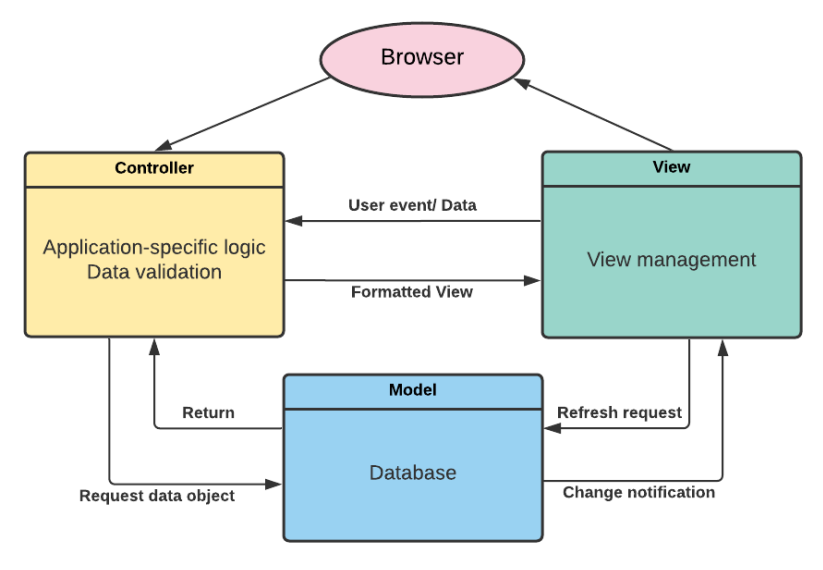
\includegraphics{Image/MVC.png}
        \caption{Mô hình kiến trúc}
    \end{figure}
    \begin{itemize}
        \item Model component
        \begin{itemize}
            \item Xác định ứng dụng sẽ có dữ liệu gì. Model component sẽ gửi thông điệp cho View khi giao diện có sự tương tác (frontend) và gửi thông điệp cho Controller khi có sự thay đổi về mặt dữ liệu của hệ thống (backend).
            \item Trong app UWC, Model sẽ mô tả những thông cần lưu trữ về nhân viên (back-officer, janitor/collector), phương tiện (troller, truck), MCPs, Route.
        \end{itemize}
        
        \item View component
        \begin{itemize}
            \item Xác định phần UI của hệ thống sẽ được hiển thị như thế nào. 
            \item Trong app UWC, View sẽ mô tả hệ thống cần render những phần nào cho người dùng như: lịch trình làm việc (work calendar) cho back-officer (dưới góc độ quản lý) và janitor/collector (dưới góc độ sử dụng), thông tin về những công việc cần làm (task info),...
        \end{itemize}
        
        \item Controller component
        \begin{itemize}
            \item Đảm nhiệm vai trò xử lý logic từ những request của người dùng và cập nhật những thông tin bên dưới database, đứng giữa View và Model.
            \item Trong app UWC, khi người dùng có yêu cầu nào đó cho hệ thống, ví dụ: yêu cầu chỉnh sửa thông tin chi tiết của một task; thì phần Controller sẽ thực hai cả hai tác vụ:
            \begin{itemize}
                \item Lấy input từ người dùng và cập nhật hiển thị lên phần UI cho người dùng thấy thông tin nào cần chỉnh sửa.
                \item Thực hiện cập nhật thông tin bên dưới phần database (nếu có yêu cầu chỉnh sửa).
            \end{itemize}
        \end{itemize}
        
    \end{itemize}
    
    
    \item \textbf{Modules} \\
\textbf{    1. Task Assignment } \\
    Task Assignment có 8 module:
    \begin{itemize}
        \item Display task on work calendar
        \item Display notifications
        \item Assign task
        \item Create notifications
        \item Task
        \item MCPs info
        \item Route
        \item Employee 
    \end{itemize}
    Các module được thể hiện như sau:\\
    \begin{figure}[!h]
    \begin{center}
      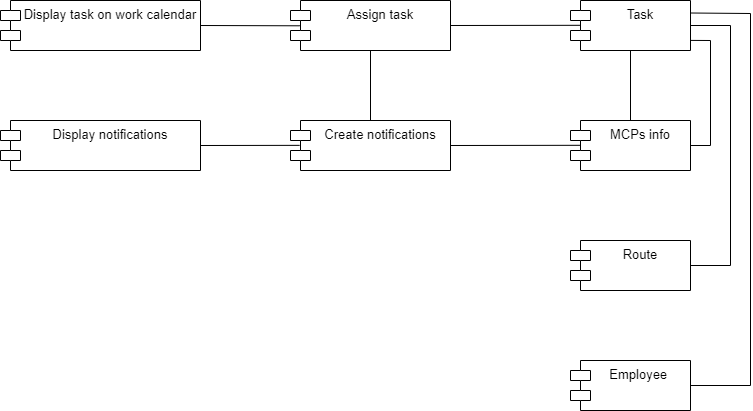
\includegraphics[width=6in]{Image/task_ass_module.png}
    \end{center}
\end{figure} \\
    Mô tả input, output, function của mỗi module\\
\textbf{    \textit{Assign task} }
    
\begin{minipage}[b]{0.4\textwidth}
Task assignment result interface có\\
- Hàm Assign\_result\_info với đầu vào là thông tin công việc (task\_info) và đầu ra là nội dung gán công việc\\
- Hàm Display\_result\_info với đầu vào nội dung gán công việc và đầu ra kiểu muốn hiển thị cho nội dung gán công việc
\end{minipage}
\hfill
\raisebox{-1\baselineskip}{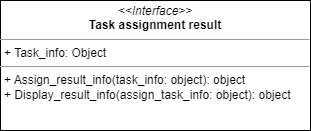
\includegraphics[width=0.5\textwidth]{Image/task_mn_1.png}}

\begin{minipage}[b]{0.4\textwidth}
Assignment result interface có \\
- Hàm Assign\_result trả về kết quả gán công việc có thành công hay không(True or False)
\end{minipage}
\hfill
\raisebox{-1\baselineskip}{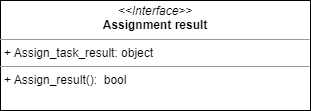
\includegraphics[width=0.5\textwidth]{Image/task_mn_2.png}}
\newpage
\textbf{\textit{Create notifications} }\\
\begin{minipage}[b]{0.4\textwidth}
Task notification interface có\\
- Hàm Notify\_content với đầu vào là kết quả gán công việc . Hàm trả về kiểu hiển thị thông báo tương ứng với kết quả đó
\end{minipage}
\hfill
\raisebox{-1\baselineskip}{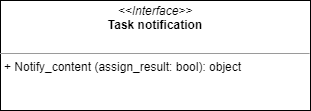
\includegraphics[width=0.5\textwidth]{Image/task_mn_3.png}}
\newline
\newline
\textbf{\textit{Employee }} \\
\begin{minipage}[b]{0.4\textwidth}
Emloyee shift list interface có \\
- Hàm Get\_employ\_shift trả về danh sách ca làm việc của công nhân
\end{minipage}
\hfill
\raisebox{-1\baselineskip}{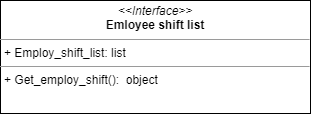
\includegraphics[width=0.5\textwidth]{Image/task_mn_5.png}}
\newline
\newline
\textbf{\textit{Route}} \\
\begin{minipage}[b]{0.4\textwidth}
Route list interface có\\
- Hàm Get\_route\_list trả về danh sách các tuyến đường
\end{minipage}
\hfill
\raisebox{-1\baselineskip}{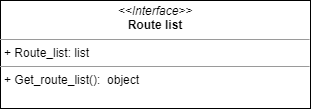
\includegraphics[width=0.5\textwidth]{Image/task_mn_6.png}}
\newline
\newline
\textbf{\textit{MCPs info}} \\

\begin{minipage}[b]{0.4\textwidth}
MCP's info list interface có \\
- Hàm Get\_mcp\_list trả về danh sách các MCP
\end{minipage}
\hfill
\raisebox{-1\baselineskip}{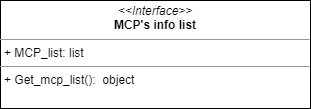
\includegraphics[width=0.5\textwidth]{Image/task_mn_7.png}}
\newline
\newline
\textbf{\textit{Task}} \\
\begin{minipage}[b]{0.4\textwidth}
Task info interface có \\
- Hàm Task\_detail trả về thông tin công việc cần gán dựa trên các thuộc tính danh sách ca làm việc của nhân viên, danh sách tuyến đường, danh sách MCP 
\end{minipage}
\hfill
\raisebox{-1\baselineskip}{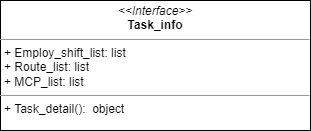
\includegraphics[width=0.5\textwidth]{Image/task_mn_4.png}}
\begin{minipage}[b]{0.4\textwidth}
New state interface có \\
- Hàm Update\_employ\_shift với đầu vào là danh sách nhân viên sau khi gán công việc(New\_employ\_shift\_list), trả về danh sách nhân viên sau khi cập nhật \\
- Hàm Update\_route với đầu vào là danh sách  tuyến đường sau khi gán công việc(New\_route\_list), trả về danh sách tuyến đường sau khi cập nhật \\
- Hàm Update\_MCP với đầu vào là danh sách  MCP sau khi gán công việc(New\_MCP\_list), trả về danh sách MCP sau khi cập nhật
\end{minipage}
\hfill
\raisebox{-1\baselineskip}{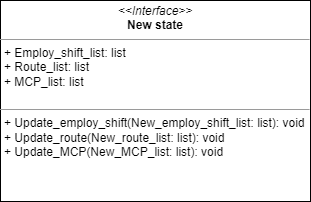
\includegraphics[width=0.5\textwidth]{Image/task_mn_8.png}}\\
\newline
\newline
\newline
\textbf{    2. MCP management } \\
    MCP management có 10 module:
    \begin{itemize}
        \item Display MCPs info
        \item Display MCP's creation
        \item Display MCP's adjustment
        \item Display notifications
        \item View MCPs
        \item Create MCPs
        \item Adjust MCPs
        \item Create notifications
        \item MCPs info
        \item Area info
    \end{itemize}
    Các module được thể hiện như sau:\\
    \begin{figure}[!h]
    \begin{center}
      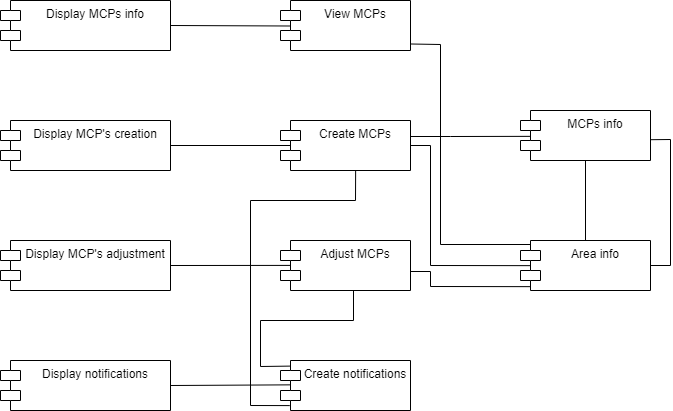
\includegraphics[width=6in]{Image/MCP_mn_md.png}
    \end{center}
\end{figure} \\
    Mô tả input, output, function của mỗi module\\
\textbf{    \textit{Area info} } \\
\begin{minipage}[b]{0.4\textwidth}
MCP info interface có \\
- Hàm Get\_MCP với đầu vào là ID của MCP. Hàm trả về MCP ứng với ID đầu vào
\end{minipage}
\hfill
\raisebox{-1\baselineskip}{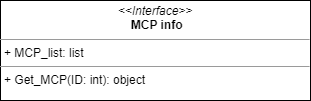
\includegraphics[width=0.5\textwidth]{Image/MCP_mn_md_3.png}}
\newpage
\begin{minipage}[b]{0.4\textwidth}
Empty MCPs list interface có \\
- Hàm Get\_empty\_MCP\_list  trả về danh sách MCP trống  danh sách các MCP
\end{minipage}
\hfill
\raisebox{-1\baselineskip}{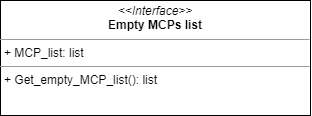
\includegraphics[width=0.5\textwidth]{Image/MCP_mn_md_1.png}}
\newline
\newline
\textbf{    \textit{MCPs info} } \\
\begin{minipage}[b]{0.4\textwidth}
Empty MCP info interface có \\
- Hàm Get\_empty\_MCP trả về MCP trống trong danh sách các MCP trống
\end{minipage}
\hfill
\raisebox{-1\baselineskip}{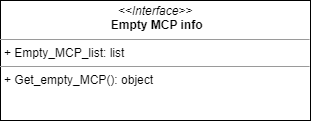
\includegraphics[width=0.5\textwidth]{Image/MCP_mn_md_2.png}}
\newline
\newline
\textbf{    \textit{View MCPs} } \\
\begin{minipage}[b]{0.4\textwidth}
  MCP info view  có \\
- Hàm Display\_MCP\_info trả về kiểu hiện hiển thị thông tin MCP
\end{minipage}
\hfill
\raisebox{-1\baselineskip}{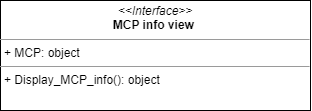
\includegraphics[width=0.5\textwidth]{Image/MCP_mn_md_6.png}}
\newline
\newline
\textbf{    \textit{Create MCPs} } \\
\begin{minipage}[b]{0.4\textwidth}
 MCP result interface có \\
- Hàm MCP\_create\_result với đầu vào là MCP rỗng. Hàm cập nhật trạng thái của MCP sang bận rộn và trả về MCP đó  \\
-  Hàm MCP\_modiy\_result với đầu vào là MCP. Hàm  điều chỉnh MCP và trả về MCP đó
\end{minipage}
\hfill
\raisebox{-1\baselineskip}{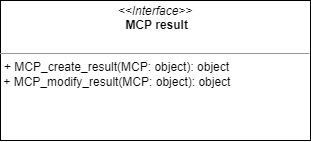
\includegraphics[width=0.5\textwidth]{Image/MCP_mn_md_4.png}}
\\ \\
\begin{minipage}[b]{0.4\textwidth}
  Result interface có \\
- Hàm Result với đầu vào là MCP sau khi thao tác. Hàm trả về kết quả thao tác MCP có thành công hay không(True or False)
\end{minipage}
\hfill
\raisebox{-1\baselineskip}{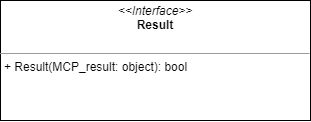
\includegraphics[width=0.5\textwidth]{Image/MCP_mn_md_5.png}}
\\ \\
\begin{minipage}[b]{0.4\textwidth}
  MCP creation result có \\
- Hàm Display\_MCP\_create trả về  kiểu hiện hiển thị nội dung MCP sau khi tạo
\end{minipage}
\hfill
\raisebox{-1\baselineskip}{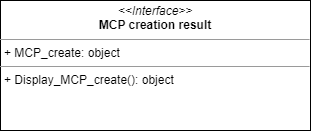
\includegraphics[width=0.5\textwidth]{Image/MCP_mn_md_7.png}}
\newline
\newline
\newpage
\textbf{    \textit{Adjust MCPs} } \\
\begin{minipage}[b]{0.4\textwidth}
 MCP result interface có \\
- Hàm MCP\_create\_result với đầu vào là MCP rỗng. Hàm cập nhật trạng thái của MCP sang bận rộn và trả về MCP đó  \\
-  Hàm MCP\_modiy\_result với đầu vào là MCP. Hàm  điều chỉnh MCP và trả về MCP đó
\end{minipage}
\hfill
\raisebox{-1\baselineskip}{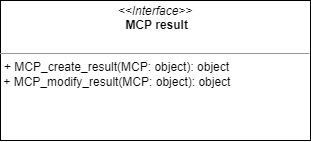
\includegraphics[width=0.5\textwidth]{Image/MCP_mn_md_4.png}}
\\ \\
\begin{minipage}[b]{0.4\textwidth}
  Result interface có \\
- Hàm Result với đầu vào là MCP sau khi thao tác. Hàm trả về kết quả thao tác MCP có thành công hay không(True or False)
\end{minipage}
\hfill
\raisebox{-1\baselineskip}{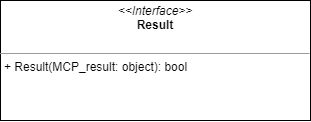
\includegraphics[width=0.5\textwidth]{Image/MCP_mn_md_5.png}}
\\ \\
\begin{minipage}[b]{0.4\textwidth}
MCP adjustment result có \\
- Hàm Display\_MCP\_adjust trả về  kiểu hiện hiển thị nội dung MCP sau khi điều chỉnh
\end{minipage}
\hfill
\raisebox{-1\baselineskip}{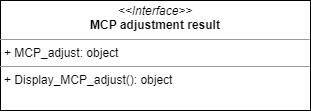
\includegraphics[width=0.5\textwidth]{Image/MCP_mn_md_8.png}}
\newline
\newline
\textbf{    \textit{MCP notification } } \\
\begin{minipage}[b]{0.4\textwidth}
MCP adjustment result có\\
- Hàm Display\_MCP\_adjust với đầu vào là kết quả tạo hoặc chỉnh sửa MCP . Hàm trả về kiểu hiển thị thông báo tương ứng với kết quả đó
\end{minipage}
\hfill
\raisebox{-1\baselineskip}{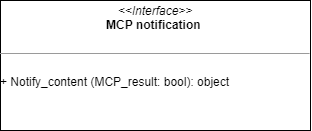
\includegraphics[width=0.5\textwidth]{Image/MCP_mn_md_9.png}}
\newline
\newline
\newline
\newpage
\textbf{    3. Communication } \\
    Communication có 8 module:
    \begin{itemize}
        \item Display message
        \item View message
        \item Search person
        \item Display search person interface
        \item Send message
        \item Message database
        \item Display notification
        \item Create notifications
    \end{itemize}
    Các module được thể hiện như sau:\\
    \begin{figure}[!h]
    \begin{center}
      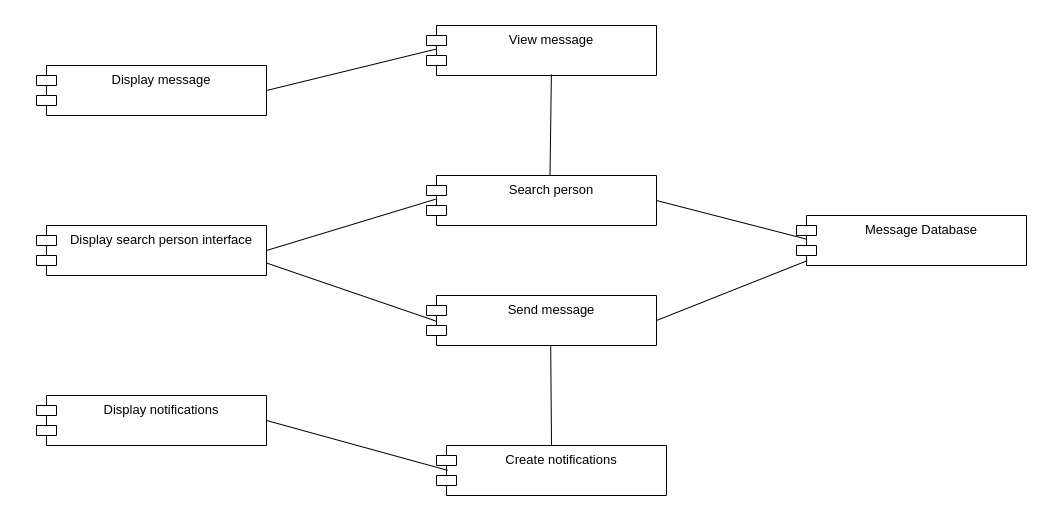
\includegraphics[width=6in]{Image/com_module.png}
    \end{center}
\end{figure} \\
    Mô tả input, output, function của mỗi module\\
\textbf{    \textit{Message database} }
    
\begin{minipage}[b]{0.4\textwidth}
Message Database cung cấp Interface "\textbf{Database connector}" - cho phép truy cập vào database, có hàm connectDatabase(), giúp kết nối với dữ liệu của hệ thống, hàm trả về true nếu kết nối thành công, và false nếu ngược lại.
\end{minipage}
\hfill
\raisebox{-1\baselineskip}{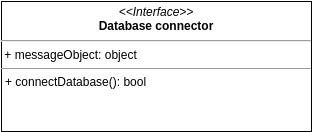
\includegraphics[width=0.5\textwidth]{Image/com_dbconnector.jpg}}
\newline
\newline
\textbf{\textit{Search person} }\\
\begin{minipage}[b]{0.4\textwidth}
- Search interface cung cấp hàm displaySearchInterce() cung cấp giao diện tìm kiếm
\end{minipage}
\hfill
\raisebox{-1\baselineskip}{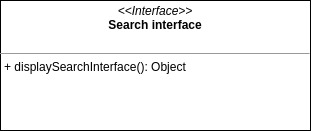
\includegraphics[width=0.5\textwidth]{Image/com_searchinterface.jpg}}
\newline
\begin{minipage}[b]{0.4\textwidth}
- Personal message có hàm getConversation() nhận vào tên người dùng và trả về dữ liệu tin nhắn của người dùng 	ứng với username đó
\end{minipage}
\hfill
\raisebox{-1\baselineskip}{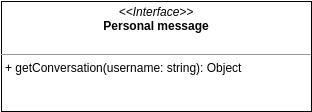
\includegraphics[width=0.5\textwidth]{Image/com_pmessage.jpg}}
\newline
\textbf{\textit{View message }} \\
\begin{minipage}[b]{0.4\textwidth}
- Interface "Message Infor" có các thuộc tính userInfo chứa thông tin về người dùng của những tin nhắn này, messageInfo là nội dung tin nhắn, và hàm displayConversation() trả về cuộc hội thoại.
\end{minipage}
\hfill
\raisebox{-1\baselineskip}{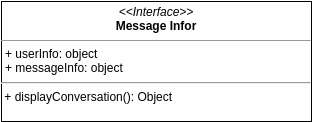
\includegraphics[width=0.5\textwidth]{Image/com_messinfor.jpg}}
\newline
\newline
\textbf{\textit{Display message}} \\
\begin{minipage}[b]{0.4\textwidth}
- Interface "Chat interface" có hàm addMessage() nhận vào một đoạn tin nhắn và trả về kết quả của về gửi tin nhắn, và hàm deleteMessage() nhận vào msgID và trả về kết quả của việc xóa một tin nhắn trong đoạn hội thoại.
\end{minipage}
\hfill
\raisebox{-1\baselineskip}{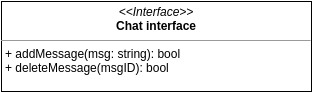
\includegraphics[width=0.5\textwidth]{Image/com_chatinterface.jpg}}
\newline
\newline
\textbf{\textit{Create notification}} \\

\begin{minipage}[b]{0.4\textwidth}
- Interface "Message notification" chứa các thuộc tính như senderName: tên của người gửi, time: thời gian gửi, và có hàm displayNotify() nhận vào trạng thái gửi tin nhắn.
\end{minipage}
\hfill
\raisebox{-1\baselineskip}{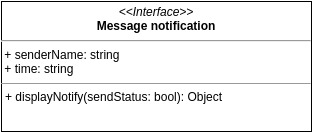
\includegraphics[width=0.5\textwidth]{Image/com_messnoti.jpg}}
\newline
\newline
\textbf{\textit{Send message}} \\
\begin{minipage}[b]{0.4\textwidth}
- Interface "Send message status" chứa trạng thái của tin nhắn (đã được gửi thành công hay chưa), và hàm getMsgStatus() trả về trạng thái của tin nhắn.
\end{minipage}
\hfill
\raisebox{-1\baselineskip}{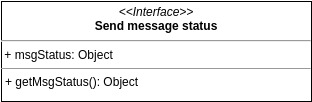
\includegraphics[width=0.5\textwidth]{Image/com_sendmessstatus.jpg}}
\begin{minipage}[b]{0.4\textwidth}
- Interface "New database state" chứa thông tin về trạng thái của tin nhắn mới được gửi, và từ đó có thể update lại database
\end{minipage}
\hfill
\raisebox{-1\baselineskip}{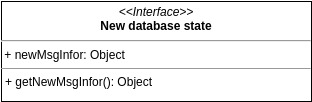
\includegraphics[width=0.5\textwidth]{Image/com_newdbstate.jpg}}\\

\newpage
\textbf{    4. Route management } \\
    Route management có 9 modules:
    \begin{itemize}
        \item Display route info
       \item Display route creation
       \item Display notifications
        \item View route
        \item Create route
        \item Optimize route
        \item Create notifications
        \item  Route info
        \item Area info
  \end{itemize}
    Các module được thể hiện như sau:\\
    \begin{figure}[!h]
    \begin{center}
      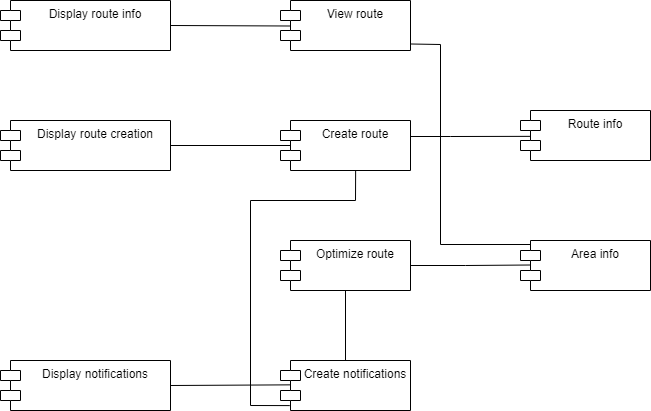
\includegraphics[width=6in]{Image/Route_Module.png}
    \end{center}
\end{figure} \\
    Mô tả input, output, function của mỗi module\\
\textbf{    \textit{Area info} } \\
\begin{minipage}[b]{0.4\textwidth}
Route info interface có \\
- Hàm Get\_route\_info với đầu vào là ID của route và trả về thông tin của route ứng với ID đó
\end{minipage}
\hfill
\raisebox{-1\baselineskip}{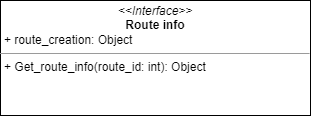
\includegraphics[width=0.5\textwidth]{Image/Route_module_1.png}}
\newpage
\begin{minipage}[b]{0.4\textwidth}
Route list interface có \\
- Hàm Get\_route\_list trả về danh sách các tuyến đường
\end{minipage}
\hfill
\raisebox{-1\baselineskip}{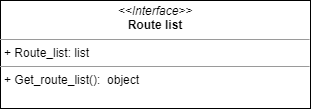
\includegraphics[width=0.5\textwidth]{Image/Route_module_2.png}}
\newline
\newline
\textbf{    \textit{Route info} } \\
\begin{minipage}[b]{0.4\textwidth}
Route info interface có \\
- Hàm Get\_route\_info với đầu vào là ID của route đã được tối ưu và trả về thông tin của route ứng với ID đó
\end{minipage}
\hfill
\raisebox{-1\baselineskip}{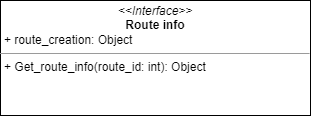
\includegraphics[width=0.5\textwidth]{Image/Route_module_1.png}}
\newline
\newline
\textbf{    \textit{View route} } \\
\begin{minipage}[b]{0.4\textwidth}
  Route info view  có \\
- Hàm Display\_route\_info trả về kiểu hiện hiển thị thông tin route
\end{minipage}
\hfill
\raisebox{-1\baselineskip}{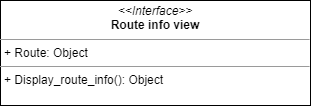
\includegraphics[width=0.5\textwidth]{Image/Route_module_3.png}}
\newline
\newline
\textbf{    \textit{Create route} } \\
\begin{minipage}[b]{0.4\textwidth}
  Route result interface có \\
- Hàm Result với đầu vào là Route sau khi được tạo. Hàm trả về kết quả tạo Route có thành công hay không(True or False)
\end{minipage}
\hfill
\raisebox{-1\baselineskip}{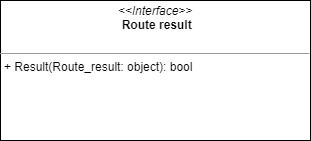
\includegraphics[width=0.5\textwidth]{Image/Route_module_4.png}}
\\ \\
\begin{minipage}[b]{0.4\textwidth}
  Route creation result có \\
- Hàm Display\_route\_creation trả về kiểu hiện hiển thị thông tin route sau khi tạo
\end{minipage}
\hfill
\raisebox{-1\baselineskip}{\includegraphics[width=0.5\textwidth]{Image/Route_module_5.png}}
\newline
\newline
\textbf{    \textit{Optimize route} } \\
\begin{minipage}[b]{0.4\textwidth}
 Route optimization result interface có \\
- Hàm Get\_optimized\_route với đầu vào là các route chưa được tối ưu.Hàm trả về các route đã được tối ưu\\
\end{minipage}
\hfill
\raisebox{-1\baselineskip}{\includegraphics[width=0.5\textwidth]{Image/Route_Module_10.png}}
\\ \\
\newline
\newline
\newpage
\textbf{    \textit{Route notifications } } \\
\begin{minipage}[b]{0.4\textwidth}
Route notifications có\\
- Hàm Notify\_content  với đầu vào là kết quả tạo. Hàm trả về hiển thị thông báo dựa trên kết kết quả đã nhận được
\end{minipage}
\hfill
\raisebox{-1\baselineskip}{\includegraphics[width=0.5\textwidth]{Image/Route_module_7.png}}
\newline
\newline
\textbf{    5. Work calendar } \\
    Route management có 8 modules:
    \begin{itemize}
     
        \item Display work calendar
        \item Display individual task info
        \item Display individual notifications
        \item Get task info
        \item Change task status
        \item Get notifications
        \item Task
        \item Notifications
 \end{itemize}
    Các module được thể hiện như sau:\\
    \begin{figure}[!h]
    \begin{center}
      \includegraphics[width=6in]{Image/cal-m.png}
    \end{center}
\end{figure} \\
    Mô tả input, output, function của mỗi module\\
\textbf{    \textit{Get task info} } \\
\begin{minipage}[b]{0.4\textwidth}
Individual calendar interface có \\
- Hàm Display\_calendar\_info trả về kiểu hiện hiển thị thông tin chung của các task
\end{minipage}
\hfill
\raisebox{-1\baselineskip}{\includegraphics[width=0.5\textwidth]{Image/cal-m1.png}}
\newpage
\begin{minipage}[b]{0.4\textwidth}
Individual tasks info interface có \\
- Hàm Display\_task\_info với đầu vào ID của task. Hiện hiển thị thông báo của task có ID tương ứng
\end{minipage}
\hfill
\raisebox{-1\baselineskip}{\includegraphics[width=0.5\textwidth]{Image/IndividualTaskInfoInterface.png}}
\newline
\newline
\textbf{    \textit{Task} } \\
\begin{minipage}[b]{0.4\textwidth}
Task info interface có \\
- Hàm Get\_task với đầu vào là ID của task. Hàm trả về task ứng với ID đầu vào
\end{minipage}
\hfill
\raisebox{-1\baselineskip}{\includegraphics[width=0.5\textwidth]{Image/cal-m3.png}}
\newline
\newline
\textbf{    \textit{Get notifications } } \\
\begin{minipage}[b]{0.4\textwidth}
Notifications có\\
- Hàm displaytNotificationList có input là id của janitor/collector và output là danh sách các notification (có đánh dấu những notification nào là mới).
\end{minipage}
\hfill
\raisebox{-1\baselineskip}{\includegraphics[width=0.5\textwidth]{Image/noti-inter.png}}
\newline
\newline
\textbf{    \textit{Notifications } } \\
\begin{minipage}[b]{0.4\textwidth}
Notification info có\\
- Hàm displayNewNotification trả về thông tin thông báo của việc thay đổi task.
\end{minipage}
\hfill
\raisebox{-1\baselineskip}{\includegraphics[width=0.5\textwidth]{Image/notifo-inter.png}}
\newline
\newline
\textbf{    \textit{Change task status} } \\
\begin{minipage}[b]{0.4\textwidth}
New status interface có \\
- Hàm Task\_new\_status với đầu vào là task với trạng thái Todo sau đó chuyển về trạng thái Ongoing và trả về.\\
- Hàm Task\_change\_result với đầu vào là task và trả về sau khi thay đổi.
\end{minipage}
\hfill
\raisebox{-1\baselineskip}{\includegraphics[width=0.5\textwidth]{Image/cal-m7.png}}
\newline
\newline

\textbf{\textit{Get individual info} } \\
\begin{minipage}[b]{0.4\textwidth}
Task info có \\
- Hàm Get task với input là ID của một task, output là task ứng với ID đó.
\end{minipage}
\hfill
\raisebox{-1\baselineskip}{\includegraphics[width=0.5\textwidth]{Image/task-inter.png}}
\newline
\newline
\end{itemize} 
\newpage
\subsection{Draw an implementation diagram for Task Assignment module}
\begin{enumerate}
    \item \textbf{Compoment Diagram - Task Assignment}
        \begin{figure}[!h]
    \begin{center}
      \includegraphics[width=6in]{Image/task_mn_arch.png}
    \end{center}
\end{figure} \\
\textbf{\textit{Mô tả}}
\begin{itemize}
\item  Khi người dùng chọn chức năng gán công việc thì khối \textit{Assign task} trong controller sẽ lấy thông tin về công việc cần gán từ khối \textit{Task} trong model. Thông tin công việc của khối \textit{Task} được tổng hợp từ các khối \textit {MCPs info},  \textit{Route},  \textit{Employee} trong model. Sau khi người dùng hoàn thành việc gán công việc thì khối \textit{Assign task} sẽ hiển thị nội dung công việc qua khối \textit{Display task on work calendar} ở view và cập nhật thông tin công việc qua khối \textit{Task} ở model
\item  Khối  \textit{Task} ở model sẽ cập nhật thông tin công việc về ca làm việc của người lao đông, MCP và các tuyến đường qua các khối tương ứng \textit{Employee },   \textit{MCPs info}, \textit{Route} ở model 
\item  Sau đó khối \textit{Assign task} sẽ gửi kết quả gán công việc qua khối \textit{Create notifications} ở controller. Khối \textit{Create notifications} sẽ hiển thị thông báo tương ứng với kết quả gán công việc qua khối \textit{Display notifications} ở view
\end{itemize}
\newpage
    \item \textbf{Compoment Diagram - MCP management}
        \begin{figure}[!h]
    \begin{center}
      \includegraphics[width=6in]{Image/MCP_mn_arch.png}
    \end{center}
\end{figure} 
\\
    \textbf{\textit{Mô tả}}
    \begin{itemize}
        \item Ta có model \textit{Area info} chứa thông tin về các MCP trong một khu vực. \textit{MCP's info} chứa thông tin về các MCP chưa được gán để xử lý, được cung cấp từ Area info. Khi người dùng muốn xem thông tin về MCP, khối controller \textit{View MCP's} sẽ lấy thông tin tất cả các MCP trong một khu vực từ khối \textit{Area Info}, sau đó cung cấp thông tin của MCP cần xem cho khối \textit{Display MCP's info} để hiển thị lên.
        \item Khi người dùng muốn Thêm thông tin về một MCP, khối controller \textit{Create MCP} sẽ lấy thông tin về các địa điểm cần gán để xử lý. Từ đó, sau khi xử lý, \textit{Create MCP} cung cấp thông tin về kết quả thêm mới MCP cho khối \textit{Display MCP's creation} để hiển thị lên màn hình, đồng thời gửi kết quả (thành công hay thất bại) về cho khối controller \textit{Create notifications}. Tương tự với khối \textit{Adjust MCP}, khối này sẽ gửi kết quả thay đổi thông tin của MCP về cho khối \textit{Display MCP's adjust} để hiển thị lên cho người dùng và cũng gửi kết quả của việc thay đổi (thành công hay thất bại) về cho khối\textit{ Create notifications}, từ đó khối \textit{Display notification} sẽ hiển thị lên thông báo kết quả của việc tạo mới/điều chỉnh. Đồng thời, cả hai khối controller này sẽ gửi kết quả điều chỉnh/tạo mới MCP về cho \textit{Area info} để cập nhật lại.
    \end{itemize}
    \newpage
    \item \textbf{Component Diagram - Communication}
    \begin{figure}[!h]
    \begin{center}
        \includegraphics[width=6in]{Image/com_componentdiagram.jpeg}
    \end{center}
    \end{figure}\\
        \textbf{\textit{Mô tả}}
    \begin{itemize}
        \item Khi người dùng sử dụng tính năng \textbf{Communication}, người dùng sẽ cần Tìm người mà mình muốn Gửi tin nhắn ở giao diện Tìm người. Khi đó, khối controller \textit{Search person} sẽ load dữ liệu về tin nhắn từ Database thông qua interface Database connector mà model \textit{Message Database} cung cấp.
        \item Khối controller \textit{View Message} sẽ sử dụng interface Personal message được cung cấp để load lên đoạn hội thoại mà người dùng có với người được tìm kiếm, sau đó khối \textit{Display Message} sẽ lấy Message Infor và hiển thị đoạn hội thoại lên màn hình.
        \item Sau đó, khối \textit{Display Message} cũng cung cấp giao diện để nhập tin nhắn cho khối controller \textit{Send Message}. Từ đó, \textit{Send Message} có thể cập nhật tin nhắn mới vào Database và gửi kết quả của việc gửi tin nhắn về cho khối controller \textit{Create notification} xử lý. Từ đó khối \textit{Display notification} có thể hiển thị thông báo đến cả người nhận và người gửi.
    \end{itemize}
        \item \textbf{Component Diagram - Route management}
        \newpage
        \begin{figure}
            \centering
            \includegraphics[width=6in]{Image/RouteManagementComponent.drawio.png}
        \end{figure}
        
        \textbf{Mô tả}
        \begin{itemize}
            \item Tính năng Route Management giúp cho cả back-officer, janitor/collector quản lý lộ trình đường đi qua những điểm cần thu gom rác về một MCP nào đó. Hệ thống hiển thị giao diện Route management thông qua View \textit{ Route Info}, được Controller \textit{View Route} lấy thông tin từ Model \textit{Area Info} ở bên dưới Database (là khu vực cần quản lý thu gom rác về một MCP).
            \item Ngoài ra, hệ thống còn cho phép back-officer có thể tạo ra tuyến đường mới qua giao diện ở \textit{Display route creation}. Controller \textit{Create route} sẽ thực hiện tác vụ tạo ra tuyến đường mới với thông tin được lấy từ Model \textit{Routes Info}. Hệ thống còn hỗ trợ tìm ra được tuyến đường tối ưu nhất (về mặt giao thông, quãng đường...) qua Controller \textit{Optimize route}. Thông tin về những tuyến đường khả thi được lấy từ một danh sách các tuyến đường từ \textit{Area info} (một khu vực có thể có nhiều tuyến đường khả thi) là chọn ra tuyến đường tối ưu nhất. Thông tin về tuyến đường đó sẽ được lưu lại bên dưới Model \textit{Routes Info}.
            \item Khi có một tuyến đường mới được tạo ra từ Controler \textit{Create route}, hệ thống sẽ gửi thông điệp tới một Controller mới tên là \textit{Create notification}. Controller nào sẽ tạo ra một thông báo mới về tuyến đường đi cho người dùng và hiển thị ở \textit{Display notification} cho người dùng biết.
        \end{itemize}
     \item \textbf{Component Diagram - Work calendar}
     \newpage
     \begin{figure}[!h]
         \begin{center}
              \includegraphics[width=6in]{Image/WorkCalendarComponent.drawio.png}
         \end{center}
     \end{figure}
     \textbf{Mô tả}
     \begin{itemize}
        \item Component Work Calendar mô tả work calendar dưới góc độ của janitor và collector. Janitor sẽ xem được thông tin về lịch trình làm việc của mình trên View \textit{Display work calendar}. Khi đó, Controller \textit{Get task info} sẽ lấy thông tin về task trong Model \textit{Task} ở Database để hệ thống hiển thị Work calendar.
         \item Khi sử dụng tính năng Work Calendar, janitor và collector sẽ xem được thông tin chi tiết của một task cụ thể được hiển thị lên Work Calendar (ví dụ: giao rác tới một khu vực) qua View \textit{Display individual task info}. Thông tin đó được Controller \textit{Get task info} từ Model \textit{Task} ở bên dưới phần Database.Trong quá trình làm việc, janitor/collector có thể đánh dấu một công việc nào đó được hoàn thành thông qua thao tác Check in/ Check out một task. Thao tác này sẽ gửi thông điệp đến Controller \textit{ Change task status} sẽ thay đổi trực tiếp trạng thái của một task (đã hoàn thành/ đang thực hiện/ chưa hoàn thành) ở phần Model \textit{Task} bên dưới phần Database, đồng thời Controller \textit{ Change task status} cũng sẽ gửi dữ liệu thông báo đến khối \textit{Notification} ở Model . Và hiển thị các thay đổi thông qua khối \textit{Display individual task info} ở View
         \item Khi có sự thay đổi về trạng thái của một task, hoặc task mới được tạo ra, thì Model \textit{Notification},  cung cấp dữ liệu cho Controller \textit{Get notification} và hiển thị thông báo đó qua phần \textit{Display individual information} để người dùng có thể thấy được.
 
     \end{itemize}
\end{enumerate}
\section{Task 4: Implementation – Sprint 1}
\subsection{Setting up. The team creates an online repository (github, bitbucket, etc) for version control. folders this stage, no need for a database to store all menu items, customers, etc. Data can be hard coded in code files.}
Link GitHub: \url{https://github.com/loctvl842/uwc?fbclid=IwAR0AXKtJe1XXMB4Tozi7YlE61c7uTGSrbihFYnGeZQhrJuY8OSzQSuFazA4}
\subsection{Adding documents, materials and folders for Requirement, System modelling and Architectural design. Use the selected version control system to report the changes to these files}
\subsection{Implement MVP1 – design an interface of either a Desktop-view central dashboard for Task Management for back-officers OR a Mobile-view Task assignment for Janitors and Collectors. Decide yourself what to include in  the view. Design use a wireframe tool. }
\end{document}